%===============================================================================
% LaTeX sjabloon voor de bachelorproef toegepaste informatica aan HOGENT
% Meer info op https://github.com/HOGENTTIN/latex-hogent-report
%===============================================================================

\documentclass[dutch,dit,thesis]{hogentreport}

% TODO:
% - If necessary, replace the option `dit`' with your own department!
%   Valid entries are dbo, dbt, dgz, dit, dlo, dog, dsa, soa
% - If you write your thesis in English (remark: only possible after getting
%   explicit approval!), remove the option "dutch," or replace with "english".

\usepackage{lipsum} % For blind text, can be removed after adding actual content
\usepackage{rotating}

%% Pictures to include in the text can be put in the graphics/ folder
\graphicspath{{../graphics/}}

%% For source code highlighting, requires pygments to be installed
%% Compile with the -shell-escape flag!
%% \usepackage[chapter]{minted}
%% If you compile with the make_thesis.{bat,sh} script, use the following
%% import instead:
\usepackage[chapter]{minted}
\usepackage{placeins}

\usemintedstyle{solarized-light}

%% Formatting for minted environments.
\setminted{%
    autogobble,
    frame=lines,
    breaklines,
    linenos,
    tabsize=4
}

%% Ensure the list of listings is in the table of contents
\renewcommand\listoflistingscaption{%
    \IfLanguageName{dutch}{Lijst van codefragmenten}{List of listings}
}
\renewcommand\listingscaption{%
    \IfLanguageName{dutch}{Codefragment}{Listing}
}
\renewcommand*\listoflistings{%
    \cleardoublepage\phantomsection\addcontentsline{toc}{chapter}{\listoflistingscaption}%
    \listof{listing}{\listoflistingscaption}%
}

% Other packages not already included can be imported here

%%---------- Document metadata -------------------------------------------------
% TODO: Replace this with your own information
\author{Arthur Van Ginderachter}
\supervisor{Dhr. P. Maenhaut}
\cosupervisor{Dhr. M. Robyn}
\title[]%
    {Evaluatie van alternatieven voor VMware vCenter: Een onderzoek naar verschillende managementplatformen voor Excentis}
\academicyear{\advance\year by -1 \the\year--\advance\year by 1 \the\year}
\examperiod{1}
\degreesought{\IfLanguageName{dutch}{Professionele bachelor in de toegepaste informatica}{Bachelor of applied computer science}}
\partialthesis{false} %% To display 'in partial fulfilment'
%\institution{Internshipcompany BVBA.}

%% Add global exceptions to the hyphenation here
\hyphenation{back-slash}

%% The bibliography (style and settings are  found in hogentthesis.cls)
\addbibresource{bachproef.bib}            %% Bibliography file
\addbibresource{../voorstel/voorstel.bib} %% Bibliography research proposal
\defbibheading{bibempty}{}

%% Prevent empty pages for right-handed chapter starts in twoside mode
\renewcommand{\cleardoublepage}{\clearpage}

\renewcommand{\arraystretch}{1.2}

%% Content starts here.
\begin{document}

%---------- Front matter -------------------------------------------------------

\frontmatter

\hypersetup{pageanchor=false} %% Disable page numbering references
%% Render a Dutch outer title page if the main language is English
\IfLanguageName{english}{%
    %% If necessary, information can be changed here
    \degreesought{Professionele Bachelor toegepaste informatica}%
    \begin{otherlanguage}{dutch}%
       \maketitle%
    \end{otherlanguage}%
}{}

%% Generates title page content
\maketitle
\hypersetup{pageanchor=true}

%%=============================================================================
%% Voorwoord
%%=============================================================================

\chapter*{\IfLanguageName{dutch}{Woord vooraf}{Preface}}%
\label{ch:voorwoord}

%% TODO:
%% Het voorwoord is het enige deel van de bachelorproef waar je vanuit je
%% eigen standpunt (``ik-vorm'') mag schrijven. Je kan hier bv. motiveren
%% waarom jij het onderwerp wil bespreken.
%% Vergeet ook niet te bedanken wie je geholpen/gesteund/... heeft


%%=============================================================================
%% Samenvatting
%%=============================================================================

% TODO: De "abstract" of samenvatting is een kernachtige (~ 1 blz. voor een
% thesis) synthese van het document.
%
% Een goede abstract biedt een kernachtig antwoord op volgende vragen:
%
% 1. Waarover gaat de bachelorproef?
% 2. Waarom heb je er over geschreven?
% 3. Hoe heb je het onderzoek uitgevoerd?
% 4. Wat waren de resultaten? Wat blijkt uit je onderzoek?
% 5. Wat betekenen je resultaten? Wat is de relevantie voor het werkveld?
%
% Daarom bestaat een abstract uit volgende componenten:
%
% - inleiding + kaderen thema
% - probleemstelling
% - (centrale) onderzoeksvraag
% - onderzoeksdoelstelling
% - methodologie
% - resultaten (beperk tot de belangrijkste, relevant voor de onderzoeksvraag)
% - conclusies, aanbevelingen, beperkingen
%
% LET OP! Een samenvatting is GEEN voorwoord!

%%---------- Nederlandse samenvatting -----------------------------------------
%
% TODO: Als je je bachelorproef in het Engels schrijft, moet je eerst een
% Nederlandse samenvatting invoegen. Haal daarvoor onderstaande code uit
% commentaar.
% Wie zijn bachelorproef in het Nederlands schrijft, kan dit negeren, de inhoud
% wordt niet in het document ingevoegd.

\IfLanguageName{english}{%
\selectlanguage{dutch}
\chapter*{Samenvatting}

\selectlanguage{english}
}{}

%%---------- Samenvatting -----------------------------------------------------
% De samenvatting in de hoofdtaal van het document

\chapter*{\IfLanguageName{dutch}{Samenvatting}{Abstract}}

Dit onderzoek richt zich op het evalueren van alternatieven voor VMware vCenter als managementplatformsysteem. Het onderzoek wordt uitgevoerd naar aanleiding van de beslissing van VMware (het bedrijf achter VMware vCenter) om de licentiekosten te verhogen. Als gevolg hiervan is Excentis op zoek naar een mogelijk alternatief voor VMware vCenter, aangezien de prijzen te hoog zijn geworden om nog rendabel te zijn voor Excentis. Door deze actie van VMware is niet alleen Excentis op zoek naar een alternatief, maar ook andere bedrijven.
De mogelijke alternatieven worden onderverdeeld in twee groepen: de open-source alternatieven en de betalende alternatieven (closed-source). Wat bieden de verschillende alternatieven aan en wat zijn de voor- en nadelen van deze alternatieven? De alternatieven worden beoordeeld op het gebied van high availability, de integratie met verschillende storage systemen, de ondersteunde hypervisors en de verschillen daartussen.
Alle geselecteerde managementplatformen die in dit onderzoek worden bekeken, zullen worden geïnstalleerd en getest in de testomgeving van Excentis in de serverruimte. Hierbij zullen verschillende aspecten worden onderzocht, de bestaande hardware en ondersteuning, performance en stabiliteit, integratie met de bestaande omgeving en werking met verschillende storage systemen. Het onderzoek zal een volwaardig alternatief bieden voor het huidige systeem dat Excentis op dit moment gebruikt met VMware vCenter.
Uiteindelijk komen er 3 geselecteerde systemen uit de selectie. De 3 systemen die zullen worden getest zijn Proxmox VE, Xen Orchestra en XenServer.
Bij deze systemen wordt er gekeken naar storage mogelijkheden voor high availability met iSCSI en distributed storage. Fibre Channel is ook een oplossing maar wordt niet verder uitgewerkt door de dure kost en beperkte mogelijkheden binnen de proof of concept.
Uit het storage gedeelte blijkt dat Proxmox en Xen Orchestra uitblinken op vlak van het aanbieden van een correct distributed storage systeem. XenCenter biedt enkel een iSCSI block based storage integratie, de laatste wordt ook aangeboden door Proxmox VE en Xen Orchestra.
Op vlak van high availability integratie bieden alle 3 de platformen een eenvoudige implementatie aan. Proxmox VE presteert wel het snelste bij een failover ten opzichte van de andere 2 systemen.
Er wordt ook gekeken hoe de virtual management platformen presteren bij het live migreren van een virtuele machine tussen 2 nodes. Hierbij bieden alle 3 de platformen een mogelijkheid aan.
Het valt op dat virtuele machines verbonden aan de distributed storage veel sneller migreren dan virtuele machines verbonden aan een externe SAN met iSCSI. Bij XenCenter is er geen integratietest gebeurd bij migreren van een VM met distributed.
Host disk swappen blinkt Proxmox VE volledig uit met een volledige integratie binnen de webinterface. Hierbij moet er geen enkele keer rechtstreeks ingelogd worden via de console op de fysieke node voor verdere configuratie van de nieuwe schijf.
Uiteindelijk komt Proxmox VE als beste uit de bus, globaal gezien op vlak van gebruiksvriendelijkheid, community, integratie met storage systemen en high availability.
Mogelijke uitbreidingen zijn ook nog te bekijken. Een goede optie die verder onderzocht kan worden, is Kubevirt, waarbij binnen Kubernetes aan virtualisatie wordt gedaan.

%---------- Inhoud, lijst figuren, ... -----------------------------------------

\tableofcontents

% In a list of figures, the complete caption will be included. To prevent this,
% ALWAYS add a short description in the caption!
%
%  \caption[short description]{elaborate description}
%
% If you do, only the short description will be used in the list of figures

\listoffigures

% If you included tables and/or source code listings, uncomment the appropriate
% lines.
\listoftables

% \listoflistings

% Als je een lijst van afkortingen of termen wil toevoegen, dan hoort die
% hier thuis. Gebruik bijvoorbeeld de ``glossaries'' package.
% https://www.overleaf.com/learn/latex/Glossaries

%---------- Kern ---------------------------------------------------------------

\mainmatter{}

% De eerste hoofdstukken van een bachelorproef zijn meestal een inleiding op
% het onderwerp, literatuurstudie en verantwoording methodologie.
% Aarzel niet om een meer beschrijvende titel aan deze hoofdstukken te geven of
% om bijvoorbeeld de inleiding en/of stand van zaken over meerdere hoofdstukken
% te verspreiden!

%%=============================================================================
%% Inleiding
%%=============================================================================

\chapter{\IfLanguageName{dutch}{Inleiding}{Introduction}}%
\label{ch:inleiding}

\section{\IfLanguageName{dutch}{Probleemstelling}{Problem Statement}}%
\label{sec:probleemstelling}

Door de aankondiging van VMware om de licentiekosten te verhogen~\autocite{device42_2024}, zijn er bedrijven die beginnen te denken aan een eventueel alternatief voor VMware ESXi/VMWare vCenter.
Hierdoor wordt dit onderzoek gevoerd. Specifiek gaan we voor het bedrijf Excentis op zoek naar een alternatief voor VMware vCenter.
Excentis is een middel groot bedrijf dat zich specialiseert in het testen van netwerken en het ontwikkelen van software voor de telecomindustrie \autocite{Excentis}.
Zij hebben enorm veel baat bij een stabiel en performant managementplatform voor virtualisatie. Een groot deel van hun omgeving draait op VMware vCenter.
De prijzen voor deze software zijn zo hoog~\autocite{Hale2024} dat bedrijven zoeken naar alternatieven.
Hoe groot zijn de kostenstijgingen en wat zijn de gevolgen voor bedrijven die gebruik maken van VMware ESXi/VMware vCenter?
Deze kosten kunnen bij bedrijven zoals Excentis zo hoog oplopen dat de kosten niet meer in verhouding staan tot de voordelen.
Welke risico's zijn er verbonden aan het blijven werken met VMware ESXi/VMware vCenter?
Zijn deze risico’s van een zodanige aard dat ze de dagelijkse werking van Excentis in de toekomst in gevaar zouden kunnen brengen?

Direct Attached Storage en Serial Attached SCSI worden bij Excentis gebruikt in combinatie met VMware vCenter.
Deze moeten ook worden overgezet naar het nieuwe alternatieve systeem. Dit zal een belangrijk criterium en onderdeel van het onderzoek zijn.

Vaak gaat het om bedrijven die virtualisatie hebben als een service, waarbij dit niet de allerbelangrijkste zorg is binnen het bedrijf.
VMware-producten zitten hard vastgeworteld in bedrijven doordat ze werken met verschillende automatisatietools en scripts. Zo'n overgang naar een nieuwe managementplatform zal een impact hebben op elke IT-infrastructuur.
Om deze overgang ook vloeiend te kunnen laten lopen, moet er in het managementplatform ook ondersteuning zijn voor onder andere Ansible automatisatietools, Nakivo en Foreman.
De mensen binnen IT moeten hierbij ook een omscholing krijgen of zich gaan verdiepen in de managementplatformen  voor virtualisatie. De documentatie en support/community achter de managementplatformen is zeker een aspect dat in rekening moet worden genomen.
Deze bachelorproef richt zich op het bedrijf Excentis: Welke alternatieven zijn er om het huidige VMware vCenter te vervangen en hoe kan die passen binnen de noden van de omgeving van Excentis?
De volgende vragen moeten worden gesteld bij het zoeken naar alternatieven op de markt.


\section{\IfLanguageName{dutch}{Onderzoeksvraag}{Research question}}%
\label{sec:onderzoeksvraag}

Evaluatie van alternatieven voor VMware vCenter: Een onderzoek naar verschillende managementplatformen met ondersteuning voor Nakivo, Ansible, en Foreman binnen Excentis
\newline De volgende deelvragen zullen beantwoord worden om de centrale onderzoeksvraag te beantwoorden:
\begin{enumerate}
  \item Welke functionele en prestatieverschillen zijn er tussen open-source en closed-source managementplatformen, en welke voor- en nadelen hebben deze verschillen voor het bedrijf Excentis?
  \item In welke mate integreren managementplatformen met tools zoals Nakivo, Ansible en Foreman, en hoe kunnen deze toegepast worden binnen Excentis?
  \item Hoe presteren managementplatformen op het gebied van High Availability(failover,\newline schaalbaarheid,backups,...)?
  \item Hoe kan de bestaande ondersteuning van Direct Attached Storage en Serial Attached SCSI in VMWare vCenter worden overgezet naar een alternatief managementplatformen binnen de infrastructuur van Excentis?
  \end{enumerate}
  
\section{\IfLanguageName{dutch}{Onderzoeksdoelstelling}{Research objective}}%
\label{sec:onderzoeksdoelstelling}
Dit onderzoek heeft als doel om een alternatief te vinden voor VMware vCenter binnen de infrastructuur van Excentis. Hierbij wordt er gekeken naar de verschillende managementplatformen die er op de markt zijn en hoe deze kunnen worden geïntegreerd binnen de infrastructuur van Excentis.
Het resultaat zal verkregen worden aan de hand van een proof of concept. Hierin zullen de specifiek geselecteerde managementplatformen uitgerold worden en de volgende criteria en testen worden uitgevoerd:
\begin{itemize}
  \item werking met de bestaande hardware van Excentis, vergeleken op prestatie en stabiliteit. (Hoe snel start een nieuwe virtuele machine op, wat zijn de minimum eisen voor de hardware, ...).
  \item Testen en meten van de performance en stabiliteit van de bestaande Direct Attached Storage en Serial Attached SCSI-systemen die Excentis gebruikt aan de hand van testdata op de nieuwe managementplatformen.
  \item De integratie van bepalende systemen binnen Excentis testen, zoals CI/CD-tools, op de nieuwe managementplatformen.
  \item Prestatie en stabiliteit van de managementplatformen bij piekmomenten en failovers.
  \end{itemize}
Een vergelijkende studie zal uitgevoerd worden tussen de verschillende managementplatformen en de resultaten zullen worden geanalyseerd. Hieruit zal een advies worden geformuleerd voor Excentis.
Als conclusie wordt er dan één managementplatform aanbevolen.

\section{\IfLanguageName{dutch}{Opzet van deze bachelorproef}{Structure of this bachelor thesis}}%
\label{sec:opzet-bachelorproef}

% Het is gebruikelijk aan het einde van de inleiding een overzicht te
% geven van de opbouw van de rest van de tekst. Deze sectie bevat al een aanzet
% die je kan aanvullen/aanpassen in functie van je eigen tekst.

De rest van deze bachelorproef is als volgt opgebouwd:

In Hoofdstuk~\ref{ch:stand-van-zaken} wordt een overzicht gegeven van de stand van zaken binnen het onderzoeksdomein, op basis van een literatuurstudie.

In Hoofdstuk~\ref{ch:methodologie} wordt de methodologie toegelicht en worden de gebruikte onderzoekstechnieken besproken om een antwoord te kunnen formuleren op de onderzoeksvragen.

% TODO: Vul hier aan voor je eigen hoofstukken, één of twee zinnen per hoofdstuk

In Hoofdstuk~\ref{ch:conclusie}, tenslotte, wordt de conclusie gegeven en een antwoord geformuleerd op de onderzoeksvragen. Daarbij wordt ook een aanzet gegeven voor toekomstig onderzoek binnen dit domein.

\chapter{\IfLanguageName{dutch}{Stand van zaken}{State of the art}}%
\label{ch:stand-van-zaken}

% Tip: Begin elk hoofdstuk met een paragraaf inleiding die beschrijft hoe
% dit hoofdstuk past binnen het geheel van de bachelorproef. Geef in het
% bijzonder aan wat de link is met het vorige en volgende hoofdstuk.

% Pas na deze inleidende paragraaf komt de eerste sectiehoofding.
VMware~\autocite{vmware} is een bedrijf dat zich specialiseert in virtualisatietechnologieën. De sterke prijsstijgingen van VMware zorgen ervoor dat veel bedrijven afhaken en op zoek gaan naar alternatieven~\autocite{Hale2024}. Er zijn verschillende alternatieve managementplatformen met bijhorende hypervisors.

\subsection{Hypervisors}
In het huidige systeem dat Excentis gebruikt, fungeert VMware ESXi~\autocite{vmware} als onderliggende hypervisor. Deze is closed source en werkt binnen het VMware systeem. Als alternatief voor VMware ESXI zijn er verschillende open-source hypervisors op de markt.
Een voorbeeld hiervan is 'KVM' (Kernel-based Virtual Machine)\autocite{KVM}. KVM is open source en vrij te gebruiken voor iedereen\autocite{KVM}. Microsoft Hyper-V ~\autocite{Eaton2019} wordt ook genoemd als mogelijke vergelijking met VMware ESXI~\autocite{fayyad2013benchmarking}. In dit onderzoek wordt een vergelijking gemaakt tussen verschillende hypervisors die geselecteerd zijn.
Verder in de virtualisatiewereld bestaat ook het Xen Project~\autocite{xenproject}. Dit is een open-source hypervisor die zich vooral richt op cloud computing en server virtualisatie ~\autocite{binu2011virtualization}.
XenServer~\autocite{xenserverwebsite} is ook een alternatieve software keuze voor VMware ESXI. XenServer is een commerciële hypervisor die zich richt op bedrijven en enterprise-ondersteuning biedt.
 
\subsection{managementplatformen}
Excentis gebruikt als managementplatform VMWare vCenter~\autocite{vmware}. Voor dit platform moet een alternatief worden gevonden.
Proxmox VE~\autocite{Proxmox} is een open-source managementplatform dat werkt met KVM en enterprise-ondersteuning aanbiedt voor bedrijven. Uit onderzoek van \textcite{ally2018comparative} blijkt dat Proxmox, dat gebruik maakt van KVM, zeker niet onderdoet tegenover andere closed source systemen.
OpenStack is een open-source cloud computing platform~\autocite{openstack2024}.
Deze biedt niet alleen ondersteuning voor KVM maar ook voor Xen~\autocite{oleksiuk2023comparative}.
Microsoft System Center Virtual Machine Manager (SCVMM)~\autocite{microsoftvmm2025} is een product van Microsoft en biedt een managementplatform systeem aan voor Hyper-V.
XenCenter~\autocite{xencenter2024} biedt een managementplatform aan voor XenServer~\autocite{xenserverwebsite}.

\subsection{Open source systemen}
Er zijn vele soorten softwarepakketten op de markt die hypervisors en managementplatformen aanbieden. Bij het bekijken van de verschillende managementplatformen met hun bijbehorende hypervisors kunnen deze worden onderverdeeld in twee groepen: de closed-source en open-source hypervisors. Elke groep heeft zijn voor- en nadelen. Alles hangt steeds af van de noden en vereisten van het bedrijf of instelling.
Proxmox VE is open source~\autocite{Proxmox}. Dit wil zeggen dat de systemen kosteloos gebruikt kunnen worden. Support bij problemen valt hierbij wel af. Er is wel een mogelijkheid om bij hen een enterprise support services subscription te nemen. Hierbij kan er alsnog beroep worden gedaan op support bij eventuele problemen.
Open source software is een evidentie maar zorgt voor meer zelfstandig werk bij installatie en rust meer op de community achter de software.

\subsection{closed source systemen}
Andere alternatieven zijn closed-source. Hierbij gaat het onder andere om VMware ESXi/VMware vCenter~\autocite{vmware} en Microsoft Hyper-V~\autocite{Eaton2019}. Deze software systemen zijn niet gratis en vragen een licentie om te mogen gebruiken. Dit is een nadeel ten opzichte van open-source systemen.
Bij bedrijven waar stabiliteit en betrouwbaarheid hoog in het vaandel staan, zoals in een wetenschappelijke omgeving met supercomputers die veel geld kosten als ze niet draaien, kan het een goede keuze zijn om te kiezen voor closed-source hypervisors~\autocite{voras2012early}. Dit wil niet zeggen dat andere systemen uitgesloten zijn.


\subsection{Soorten storage systemen}
Wanneer het over opslag in de virtualisatiewereld gaat, betreft het ook 'Serial-Attached SCSI' (SAS) en 'Direct-Attached Storage' (DAS). Deze technologieën zorgen ervoor dat er een hoge beschikbaarheid is van de data en dat deze snel kan worden opgevraagd~\autocite{griswold2002storage}. Dit is een belangrijk aspect in de virtualisatiewereld en is belangrijk voor Excentis dat deze beide technologieën perfect werken en ondersteunt worden.
SAS is een snelle, betrouwbare opslaginterface die servers en high-performance opslagapparaten verbindt~\autocite{aravindan2014performance}. Dit is een belangrijk om een consistente opslag te garanderen. DAS is een opslagarchitectuur waarbij opslag direct fysiek is verbonden aan een enkele server, zonder tussenkomst van een netwerk. Deze technologie is goedkoper en eenvoudiger, maar garandeert niet alle voordelen die SAS wel kan garanderen~\autocite{griswold2002storage}.
DAS wordt vaak gebruikt in kleinere bedrijven waar de data niet zo belangrijk is en waar de data niet zo vaak wordt opgevraagd. SAS wordt vaak gebruikt in grotere bedrijven waar de data zeer belangrijk is en waar de data vaak wordt opgevraagd~\autocite{griswold2002storage}.
Zo goed als alle managementplatformen ondersteunen DAS en SAS in ons onderzoek. Excentis wilt weten hoe deze ondersteuning kan worden overgezet naar een nieuw managementplatform.

Storage Area Network (SAN) \textcite{ibm2025san} is een technologie die gebruikt wordt om storage te delen over het netwerk.
Dit is puur een manier om storage op te zetten.
Je hebt hiernaast ook nog een protocol of manier nodig om te kunnen communiceren met de storage op die server.


\subsection{High Availability-ondersteuning}
In het onderzoek van~\textcite{dudnik2017creating} wordt een grote vergelijking gemaakt tussen hypervisors en hun managementplatformen. Hierin wordt gefocust op bepaalde aspecten binnen de term High Availability, zoals redundantie, risicoanalyse en piekdrukte.
Er zijn verschillende aspecten die moeten worden bekeken en waaraan voldaan moet worden om aan een goede High Availability te voldoen. Een failover-systeem dat het ene systeem het andere systeem over laat nemen bij een bepaalde fout, is een van die aspecten.
Op netwerkniveau moet er ook nagedacht worden over zowel schaalbaarheid bij piekmomenten als bij problemen die zich voordoen in het netwerk. Migratie tussen verschillende fysieke servers moet ook mogelijk zijn om een goede High Availability te garanderen~\autocite{dudnik2017creating}.
Workloadmanagers kunnen een goede oplossing zijn om overbelasting tegen te gaan op drukke piekmomenten. Back-ups van de data worden ook gezien als een belangrijk aspect voor High Availability.


\subsection{samenvatting van alle managementplatformen en hun bijhorende hypervisors}
    \begin{table}[h!]
        \centering
        \begin{tabular}{|l|l|l|l|}
        \hline
        \textbf{Platform}      & \textbf{Type}      & \textbf{Hypervisor} & \textbf{Description} \\ \hline
        VMware vCenter         & Closed-source      & VMware ESXi         & Enterprise management platform voor VMware-gebaseerde virtualisatie. \\ \hline
        Microsoft SCVMM        & Closed-source      & Microsoft Hyper-V   & Beheert Hyper-V-omgevingen en biedt integratie met andere Microsoft-producten. \\ \hline
        Proxmox VE             & Open-source        & KVM                 & Geavanceerd open-source managementplatform voor KVM, met enterprise-ondersteuning. \\ \hline
        OpenStack              & Open-source        & KVM, Xen            & Cloud computing-platform dat meerdere hypervisors ondersteunt. \\ \hline
        XenCenter              & Closed-source      & XenServer           & Managementplatform specifiek ontworpen voor XenServer-gebruikers. \\ \hline
        Xen Project            & Open-source        & Xen                 & Managementplatform dat Open-source is. \\ \hline
        \end{tabular}
        \caption{Vergelijking van Virtualisatieplatforms}
        \end{table}
        
\subsection{Prestatie verschillen tussen XenServer en Proxmox VE}
In het onderzoek van \textcite{algarni2018performance} wordt een vergelijkende studie gemaakt tussen Xen en KVM. In ons onderzoek focussen wij ons vooral op het managementplatform.
Aangezien een managementplatform ook een hypervisor nodig heeft kunnen wij hier spreken over het management platform die gekoppeld is in deze studie aan een hypervisor.
Voor KVM spreken we over PROXMOX VE en voor Xen spreken we over XenServer. In deze studie wordt er een vergelijking gemaakt tussen de twee systemen en hun prestaties. De resultaten zijn als volgt:

\begin{itemize}
    \item Proxmox VE heeft een betere prestatie in termen van CPU-gebruik en geheugengebruik dan XenServer.
    \item XenServer heeft een betere prestatie in termen van I/O-prestaties dan Proxmox VE zoals bestandssysteem beheer en applicatie prestaties.
\end{itemize}                               
Over het volledige onderzoek van \textcite{algarni2018performance} heen krijg KVM (gekoppeld aan Proxmox VE voor ons onderzoek) de beste punten over het globael punt heen. Dit onderozek heeft plaats gevonden in 2018 waarbij de conclusies nog alst actueel kunnen beschouwd worden.
Dit is een belangrijk onderzoek om conclusies uit te trekken eenmaal een proof of concept gemaakt is.

\subsection{Storage ondersteuning voor hypervisors en managementplatformen}

Zoals eerder uitgelegd wordt er in dit onderzoek gekeken naar Serial-Attached SCSI (SAS) en Direct-Attached Storage (DAS). Deze technologieën zijn belangrijk voor de virtualisatiewereld en zijn ook belangrijk voor Excentis. Het is belangrijk dat deze technologieën goed werken met de hypervisors en managementplatformen die in dit onderzoek worden bekeken.
Om in de proof of concept deze technologieën te kunnen gebruiken moet er gekken worden of elk managamentplatform deze technologieën ondersteunt.
SAS-storage staat los van elke hypervisor met hun bijhorende virtual managementplatformen.

\begin{figure}[h!]
    \centering
    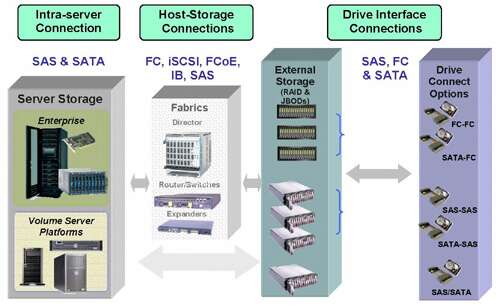
\includegraphics[width=0.7\textwidth]{../onderzoek/storagesas-das.jpg} 
    \caption{volledig beeld die SAS weergeeft, afkomstig van \href{https://www.eetimes.com/serial-attached-scsi-storage-moves-ahead-in-network-server-designs/}{eetimes}.}
    \label{fig:sas}
\end{figure}

\FloatBarrier
De onderstaande figuur toont de kracht van SAS systemen. In het artikel van \textcite{loshin2022sas} wordt er uitgelegd dat SAS tot 2 keer zoveel meer data kan versturen en verwerken t.o.v. het bekende SATA systeem.

\begin{figure}[h!]
    \centering
    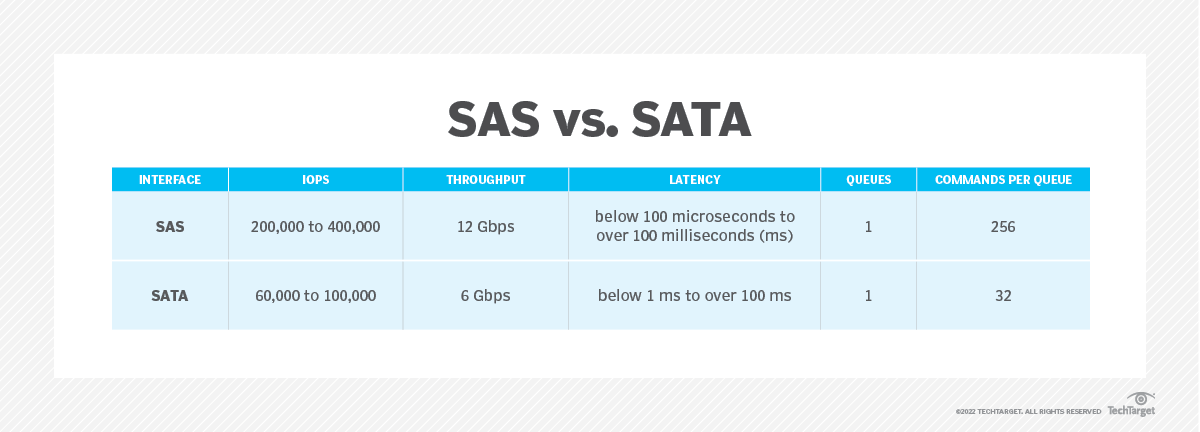
\includegraphics[width=0.7\textwidth]{../onderzoek/sas_vs_sata-f.png} 
    \caption{Afbeelding die SAS prestatie weergeeft, afkomstig van \href{https://www.techtarget.com/searchstorage/definition/serial-attached-SCSI}{TechTarget} over Serial Attached SCSI.}
    \label{fig:saspres}
\end{figure}


\FloatBarrier
Verder wordt er ook nog Storage Area Network (SAN) gebruikt in combinatie met iSCSI voor grote storage-opslagsystemen. In het onderzoek van \textcite{park2024performance} wordt besproken hoe iSCSI een positieve invloed heeft op de prestatie van storagesystemen die gedeeld worden met verschillende toepassingen.
In het bedrijf Excentis is het daarom ook belangrijk dat de storage van het virtual managementplatform gedeeld kan worden met verschillende toepassingen. Bij het onderzoek van \textcite{park2024performance} wordt bevestigd dat dit een goede standaardmethode is voor storage over het netwerk.
ISCI is hiermee ook een belangrijk punt om rekening mee te houden in de proof of concept. Het is belangrijk dat de iSCSI goed werkt met de hypervisors en managementplatformen die in dit onderzoek worden bekeken.

\begin{figure}[h!]
  \centering
  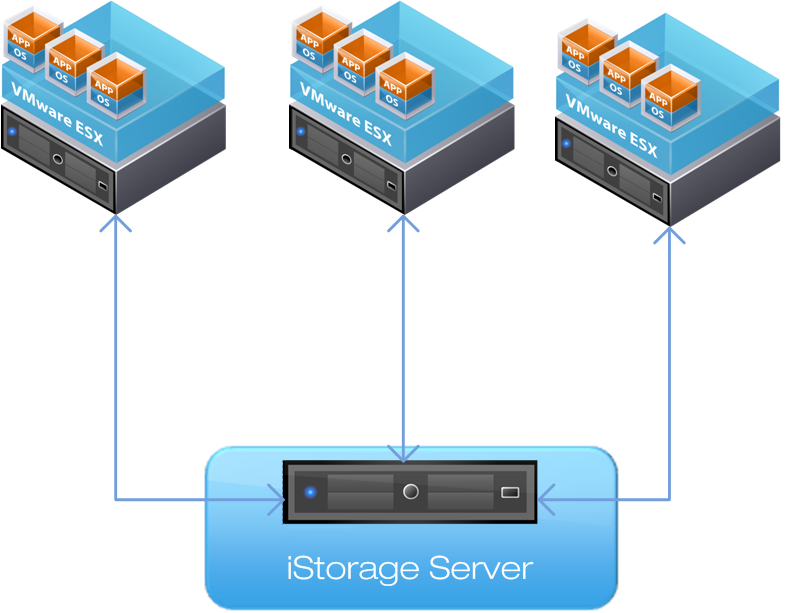
\includegraphics[width=0.7\textwidth]{../onderzoek/nas-isci.png} 
  \caption{Afbeelding die SAN simpel weergeeft, afkomstig van \href{https://www.kernsafe.com/images/VMware-iSCSI-iStorage-Server.png}{kernsafe}.}
  \label{fig:san}
\end{figure}


\FloatBarrier
Bij DAS-systemen wordt, zoals eerder vermeld, de data rechtstreeks aan de hardware verbonden. Het onderzoek van \textcite{joshi2014empirical} richt zich specifiek tot schijfformaten op DAS-systemen.
Dit gaat buiten de scope van dit onderzoek, maar toont zeer mooi aan dat KVM (voor ons Proxmox VE) zeer goede ondersteuning biedt en hierbij ook aantoont dat er zeer veel ondersteunende schijfformaten bestaan.
Het is zeer moeilijk om correcte wetenschappelijke artikels te vinden over implementatie van DAS- en SAS-systemen op alle soorten managementplatformen. Er wordt vaak specifiek gericht op een gebruikt systeem die zich onder de categorie bevindt DAS of SAS. Het onderzoek van \textcite{joshi2014empirical} is daar een goed voorbeeld van.
Met de referenties en kennis die hieruit zijn gekomen, weten we dat DAS en SAS globaal over alle managementplatformen ondersteund worden. De uitvoering en de praktische ervaring zal in de proof of concept worden bekeken. Daaruit moet uitkomen of de SAS- en DAS-integratie voldoende stabiliteit biedt.

\begin{figure}[h!]
    \centering
    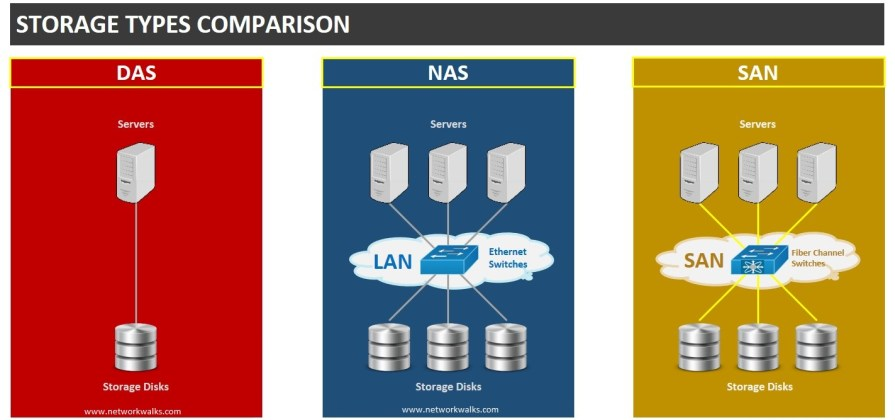
\includegraphics[width=0.7\textwidth]{../onderzoek/DAS.jpg} 
    \caption{Afbeelding die DAS simpel weergeeft, afkomstig van \href{https://networkwalks.com/storage-types-das-nas-san/I}{Networkwalks}.}
    \label{fig:das}
\end{figure}
\FloatBarrier
gedistribueerde opslag of distributed storage is nog een belangrijke optie die toepasselijk is voor een virtual managementplatform. Dit is een opslagmethode waarbij de data over verschillende servers (nodes) wordt verdeeld. Dit zorgt ervoor dat de data sneller kan worden opgevraagd en netwerk verkeer eficient benut wordt. ~\autocite{patil2010unified}.
In het onderzoek zijn wij specifiek gefocust op toepassingen voor management platformen. VMware heeft izjn eigen private toepassing genaamd VSAN~\autocite{hogan2016essential}. Dit is een software-defined storage oplossing die speciaal is ontworpen voor VMware-omgevingen. Het biedt een effectieve opslagoplossing die eenvoudig kan worden geïntegreerd met VMware's virtualisatieplatforms.
Hierbij moet er dus ook een alternatief ter beschikking zijn. Een daarvan die open source is, is Ceph~\autocite{weil2006ceph}. Dit is een open-source software-defined storage oplossing die kan worden gebruikt met verschillende managementplatformen zoals Proxmox VE ~\autocite{Proxmox}.

Hieronder is een theoretisch voorbeeld aangetoont. Ceph zelf en VSAN kan je vergelijken met dit theoretisch voorbeeld.
\begin{figure}[h!]
  \centering
  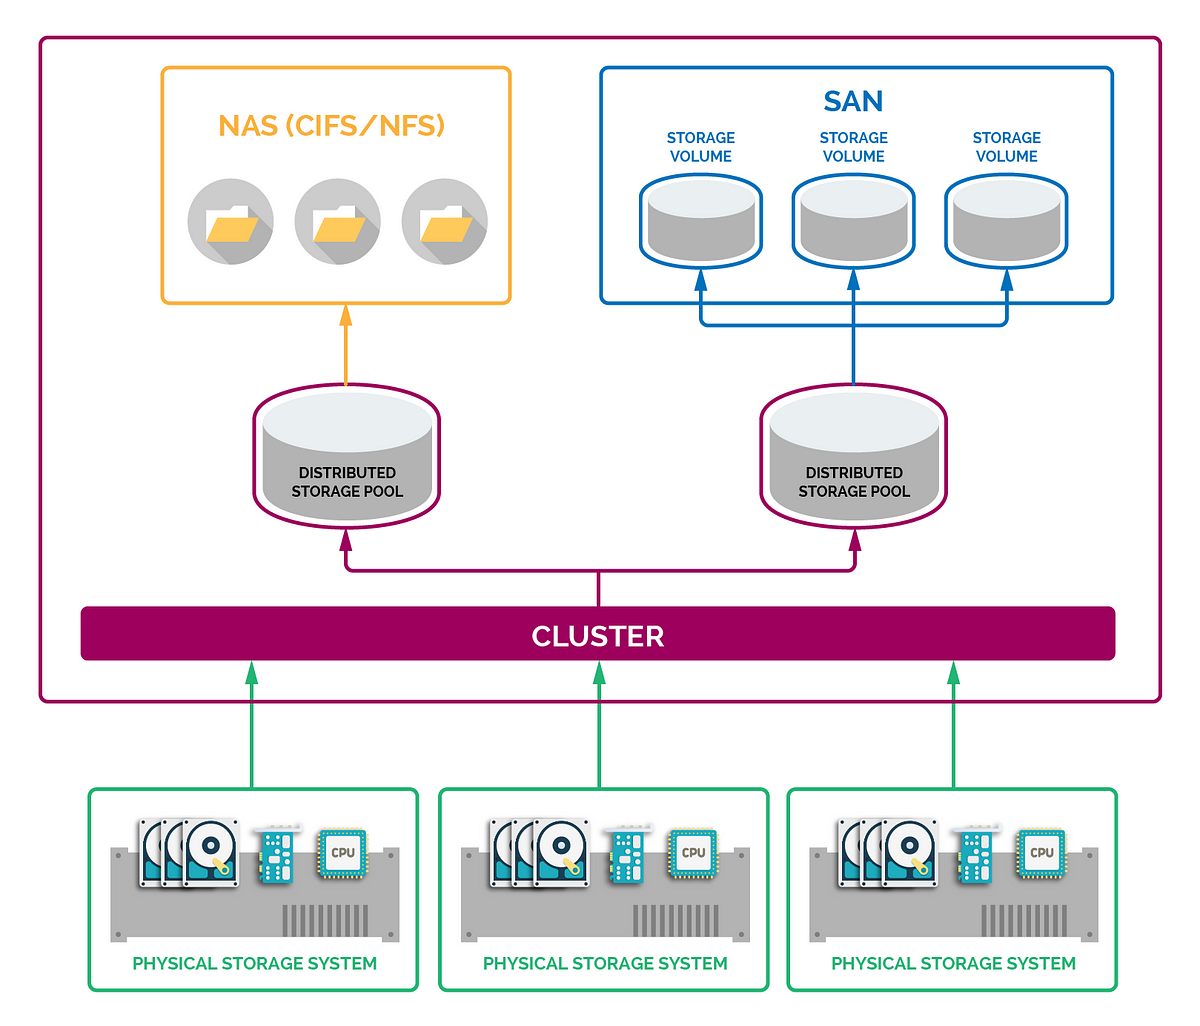
\includegraphics[width=0.9\textwidth]{../onderzoek/dssep.png} 
  \caption{Afbeelding van distributed storage als toepassing., afkomstig van \href{https://medium.com/systemdesign-us-blog/how-does-storage-work-in-distributed-systems-fde890e88a7f}{Medium}.}
  \label{fig:das}
\end{figure}
%%=============================================================================
%% Methodologie
%%=============================================================================

\chapter{\IfLanguageName{dutch}{Methodologie}{Methodology}}%
\label{ch:methodologie}

%% TODO: In dit hoofstuk geef je een korte toelichting over hoe je te werk bent
%% gegaan. Verdeel je onderzoek in grote fasen, en licht in elke fase toe wat
%% de doelstelling was, welke deliverables daar uit gekomen zijn, en welke
%% onderzoeksmethoden je daarbij toegepast hebt. Verantwoord waarom je
%% op deze manier te werk gegaan bent.
%% 
%% Voorbeelden van zulke fasen zijn: literatuurstudie, opstellen van een
%% requirements-analyse, opstellen long-list (bij vergelijkende studie),
%% selectie van geschikte tools (bij vergelijkende studie, "short-list"),
%% opzetten testopstelling/PoC, uitvoeren testen en verzamelen
%% van resultaten, analyse van resultaten, ...
%%
%% !!!!! LET OP !!!!!
%%
%% Het is uitdrukkelijk NIET de bedoeling dat je het grootste deel van de corpus
%% van je bachelorproef in dit hoofstuk verwerkt! Dit hoofdstuk is eerder een
%% kort overzicht van je plan van aanpak.
%%
%% Maak voor elke fase (behalve het literatuuronderzoek) een NIEUW HOOFDSTUK aan
%% en geef het een gepaste titel.

\subsection{Literatuurstudie en voorbereidend onderzoek}
Een objectief resultaat van alle managementplatformen is gewenst om deze vervolgens naast elkaar te kunnen vergelijken. Om dit te bereiken, wordt een vergelijkende studie uitgevoerd.De verschillende managementplatformen worden met elkaar vergeleken om te bepalen welke het beste aansluit bij de noden van Excentis.
Aan de hand van literatuurstudie en onderzoeken worden de managementplatformen geselecteerd die met elkaar worden vergeleken.
Er zal samen met Excentis worden overlopen welke eisen zeker voldaan moeten worden en wat het bedrijf echt nodig heeft in hun managementplatform, gecombineerd met hun bestaande infrastructuur. Er zal ook gekeken worden naar wat er momenteel allemaal wordt gebruikt binnen hun omgeving. Deze zullen dan worden meegenomen als basisvereisten voor de alternatieve managementplatformen.
Deze fase zal ook gebruikt worden om de testomgeving op te zetten en de hardware te voorzien die nodig is voor de testen.

\subsection{selecteren van managementplatformen met hun bijhorden hypervisor}
Er zijn verschillende soorten managementplatformen op de markt die kunnen worden getest en vergeleken. Hieruit moet er een bepaalde selectie komen waar er verder mee vergeleken kan worden voor in de proof of concept.
Aangezien de tijd en middelen beperkt zijn, is het belangrijk om hierop een goede minimumcriteria te hebben waarop de managementplatformen worden geselecteerd.

\begin{enumerate}
\item Minimaal 1 open-source managementplatform die geen betalende licentie heeft voor de software (exclusief support).
\item Er is een volwaardige supportaanbieding voor commercieel gebruik. Hierbij kan de klant mits een betalende licentie beroep doen op support bij problemen.
\item Het kan draaien op de bestaande DELL-servers die tot de beschikking zijn in de proof of concept.
\item Het managementplatform moet verschillende nodes kunnen aansturen en beheren.
\item Betalende managementplatformen die een licentie nodig hebben, bieden een gratis proefversie aan om deze studie te kunnen uitvoeren in de proof of concept-omgeving.
\end{enumerate}

Als deze criteria zijn voldaan voor een specifiek managementplatform, wordt deze geselecteerd voor te draaien in de proof of concept.

\subsection{Opzetten testomgeving/proof of concept}
De hardware en omgeving waarin alles wordt getest en opgebouwd, worden opgesteld in een testomgeving bij Excentis. Dit maakt het mogelijk om de managementplatformen te testen in een realistische omgeving, wat essentieel is om een objectief resultaat te bekomen.
Deze omgeving zal bestaan uit 2 verouderde DELL servers die in de serverruimte van Excentis staan. Hierbij zal alles op kleine schaal kunnen worden uitgevoerd.
Op deze servers worden de geselecteerde managementplatformen geïnstalleerd.
\subsection{Uitvoeren onderzoek op testomgeving}
Voor de vergelijking van de managementplatformen worden de volgende acties uitgevoerd op de testomgeving van Excentis:
\begin{itemize}
\item werking met de bestaande hardware van Excentis, vergeleken op prestatie en stabiliteit. (Hoe snel start een nieuwe virtuele machine op, wat zijn de minimum eisen voor de hardware, ...).
\item Testen en meten van de performance en stabiliteit van de bestaande Direct Attached Storage en Serial Attached SCSI-systemen die Excentis gebruikt aan de hand van testdata op de nieuwe managementplatformen.
\item De integratie van bepalende systemen binnen Excentis testen, zoals CI/CD-tools, op de nieuwe managementplatformen.
\item Prestatie en stabiliteit van de managementplatformen bij piekmomenten en failovers.
\item hot swapping van hard disks. Blijf alles correct werken? 
\item Neemt de ene node de virtuele machines over van de andere node bij een failover?
\end{itemize}

\subsection{Evalueren van de resultaten}
Deze acties worden stap voor stap uitgevoerd bij elk managementplatform, dit om een zo objectief mogelijk resultaat per managementplatform te verkrijgen.
Als alle acties zijn uitgevoerd, worden de resultaten met elkaar vergeleken en wordt er een conclusie getrokken over welk managementplatform het beste aansluit bij de noden van Excentis.

\chapter{\IfLanguageName{dutch}{Proof of concept}{Proof of concept}}%
\label{ch:poc}

\section{inleiding}%
Aan de hand van de shortlist die opgemaakt is komt er voor elke geselecteerde managementplatform een proof of concept. Hierbij wordt er gekeken hoe de nodige functionaliteiten werken en toegepast kunnen worden in het systeem.
Belangrijk om te weten is dat de proof of concept niet de volledige functionaliteit van het managementplatform zal testen. Het doel is om een goed beeld te krijgen van de mogelijkheden en hoe deze kunnen worden toegepast binnen de infrastructuur van Excentis. 
We verdelen alle managementplatformen in hun eigen subsecties. In deze subsecties worden dan de vooropgestelde testen op uitgevoerd.
\section{Proxmox VE}%
Voor deze virtual managementplatform wordt er Proxmox VE 8.4 gebruikt. Dit is de laatste versie van Proxmox VE die op dit moment beschikbaar is.
\subsection{Storage in Proxmox VE}
Ìn deze proof of concept worden er 2 storage integraties bekeken en getest.
\begin{itemize}
    \item CEPH storage
    \item SAN iSCSI (met TrueNAS ~\autocite{truenas})
\end{itemize}
In sectie \autoref{sec:storage_proxmox} wordt er dieper ingegaan op de configuratie van de storage in Proxmox VE.
CEPH wordt toegepast op alle 3 de fysieke nodes. Elk hebben hun eigen schijf die gebruikt wordt door CEPH. Deze schijven nemen elkaars taken over bij een failover of het maken van redunante data.
iSCI bij Proxmox VE biedt op een makelijke manier de mogelijkheid om een SAN te configureren. 
Beiden werden probleemloos geconfigureerd en getest bij een virtuele machine. Zie \ref{sec:storage_proxmox} voor meer details.
\subsection{High Availability in Proxmox VE}
In \autoref{sec:ha-proxmox} wordt de configuratie voor HA in detail uitgelgd.
De test zellf wordt uitgevoerd bij 2 virtuele machines die elk gekoppeld zijn aan hun eigen storage systeem (iscsi of CEPH).
Hierna worden ze toegevoegd aan een HA-groep. Dit is een groep van virtuele machines die samen prioriteit hebben in de cluster.

Om HA te testen in combinatie met beide storage systemen zal er een netwerk probleem worden gesimuleerd.
Alle virtuele machines draaien nu op node 001
Op de fysieke node poc001 zal de internet kabel worden uitgetrokken. Hierna kijken we hoelang het duurt vooraleer de virtuele machines opnieuw worden opgestart op een andere node, alsookop welke node specifiek. \\

Figuur \ref{fig:failover-vm} kan er duidelijk gezien worden dat de virtuele machines volledig van cold mode moeten opstarten. Dit is een andere situatie dan wanneer er een migratie gedaan wordt.
Dan wordt live de virtuele machine van de ene node naar de andere gemigreerd zonder echte downtime.
Het systeem in Proxmox VE is nu zo ingesteld dat bij een echte failover de schade van downtime relatief beperkt blijft. Dit staat uiteraard los van data verlies die kan optreden bij een failover.
\begin{figure}[H]
  \centering
  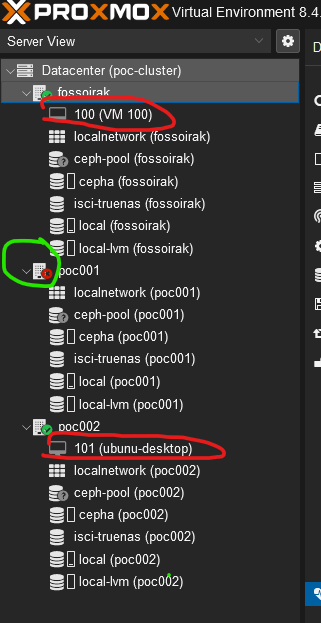
\includegraphics[width=0.55\textwidth]{../poc/failover-prox.png}
  \caption{failover node virtuale machines herstellen in HA in Proxmox VE}
  \label{fig:failover-vm}
\end{figure}

Van zodra de connectie van poc001 verboken is met de nadere nodes duurt het ongeveer 30-60 seconden vooraleer de virtuele machines opnieuw worden opgestart op een andere node. Dit is ook de tijd die nodig is om de heartbeat van de cluster te verliezen.
Hierbij kunenn we vanuit gaan dat de default healthy check van de cluster en zijn nodes ook rond deze tijdsduur ligt. Beide virtuele machines worden opnieuw opgestart op de node foissarak en poc002. \\
Aangezien beide virtuele machines dezelfde HA group hebben, krijgen ze ook dezelfde prioriteit.

Merk op dat zowel de virtuele machine met een SAN als de virtuele machine met een distributed storage opnieuw worden opgestart op de node foissarak. Dit toont aan dat Proxmox VE goed werkt met beide storage systemen, zeker met failover situaties.

\subsection{Virtuele machines migraties in Proxmox VE}
In het het werkveld komt het geregeld voor dat een node een gepland onderhoud heeft. Dit kan zijn dat er een update moet worden uitgevoerd of dat er hardware moet worden vervangen.
Bij deze is het gewenst om te weten of er een mogelijkheid is om de virtuele machines te migreren naar een andere node zonder dat er downtime/minimale downtime is.
Via de GUI in Proxmox VE kan een virtuele machine eenvoudig worden gemigreerd via de optie Migration rechtsboven, zodra een virtuele machine is geselecteerd, zie figuur \ref{fig:migratie-vm}.
\begin{figure}[H]
  \centering
  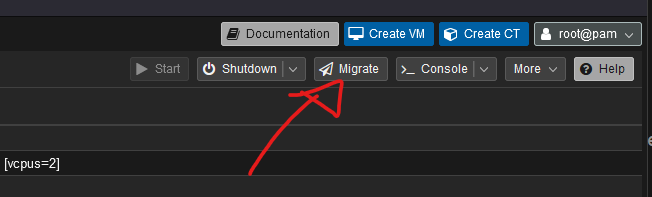
\includegraphics[width=0.85\textwidth]{../poc/vm-migratie-prox.png}
  \caption{migratie virtuele machine in Proxmox VE}
  \label{fig:migratie-vm}
\end{figure}
Tijdens het migreren van de virtuele machine blijft de console open staan van de virtuele machine. Hierbij is er een zeer korte freeze in het beeld waarna de activiteiten in de vm weer verder werken. Het totale proces voor beide virtuele machines individueel was ongeveer 30 seconden.
Hieruit kan er bekeken worden dat de downtime bij migratie zo goed als minimaal is, wat ideaal is voor het offline brengen van een node voor bijvoorbeeld een gepland onderhoud.

\subsection{Hot swapping fysieke disks in Proxmox VE}
Proxmox VE biedt ook hot swapping aan van de fysieke disks. 
Voor deze test is er een fysieke disk voor node poc002 toegevoegd, zie figuur \ref{fig:hotdisk-swap}.
\begin{figure}[H]
  \centering
  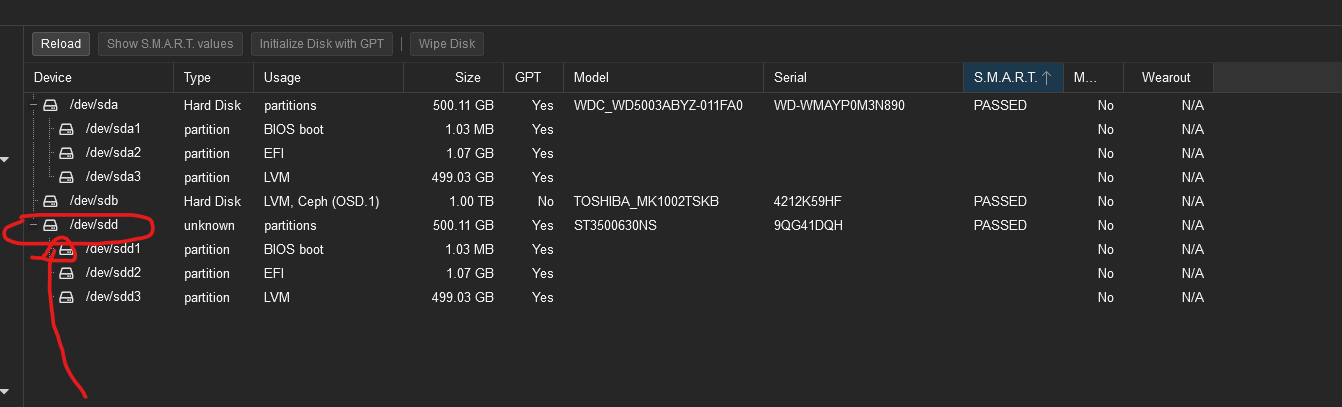
\includegraphics[width=1.2\textwidth]{../poc/hot-disk-prox.png}
  \caption{hot disk swap in Proxmox VE}
  \label{fig:hotdisk-swap}
\end{figure}
Deze noemt sdb. Eenmaal dat deze disk is toegevoegd zou de disk moeten kunnen verwijderd worden en vervangen worden door een andere zonder dat de node poc002 offline moet worden gehaald.
Dit wordt live getest tijden het draaien. Op deze disk draait momenteel niks. Dit is belangrijk aangezien we het vervangen van een disk simuleren. De data zou normaal op voorhand moeten verwijderd zijn van de disk.

We voegen de nieuwe disk toe in de plaats van de andere en merken direct na 15 seconden dit op, zie figuur \ref{fig:hotdiskvervangen-swap}.
\begin{figure}[H]
  \centering
  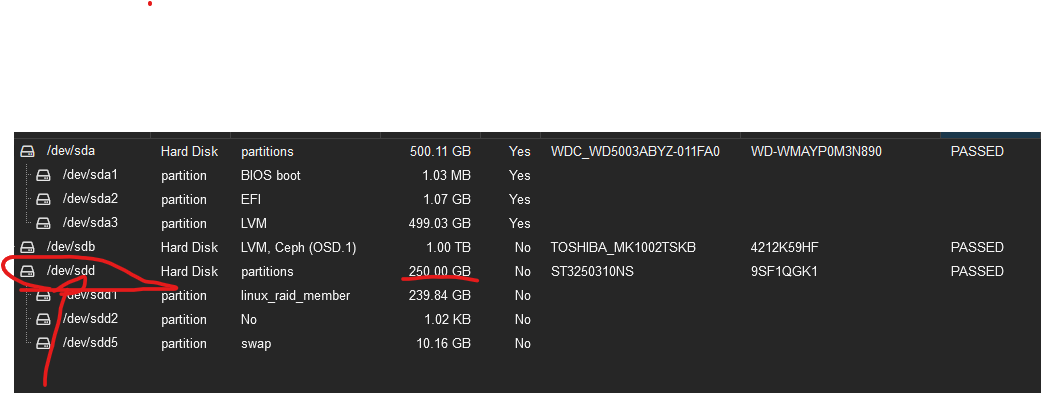
\includegraphics[width=1.2\textwidth]{../poc/hot-disktwee-prox.png}
  \caption{hot disk swap in Proxmox VE}
  \label{fig:hotdiskvervangen-swap}
\end{figure}

We zien bij figuur` \ref{fig:hotdiskvervangen-swap} dit duidelijk een andere disk is met nu een grote van 250 GB. Hiervoor was dat 500 GB.
% Voor deze virtual managementplatform wordt er Proxmox VE 8.4 gebruikt. Dit is de laatste versie van Proxmox VE die op dit moment beschikbaar is.
% \subsection{cluster opstelling in Proxmox VE}
% Voor proxmox VE is er gekozen om te werken met 3 fysieke node's. Zoals beschreven op de officiële documentatiepagina van Proxmox ondersteunt het platform high availability clustering maar moeten er minimaal 3 nodes in de cluster draaien ~\autocite{proxmoxHA}.
% Hierbij spreken we over minimaal 50\% van de nodes die moeten draaien om de cluster operationeel te houden. Dit is ook de reden waarom er voor 3 nodes is gekozen.
% Bij 2 nodes zou er bij een node failure geen quorum zijn en zou de cluster niet meer operationeel zijn. Dit wil zeggen dat er geen 50\% meerderheid is van de cluster die online is. Enkel bij 3 nodes kan er 1 node uitvallen en alsnog meer dan 50 procent online hebben. In zo een gavel spreken we van een quorum.
% In de figuur \ref{fig:cluster-proxmox} wordt de opstelling getoond. Elke node heeft zijn unieke naam in de cluster, vaak is dat de hostname zelf.
% \begin{figure}[H]
%   \centering
%   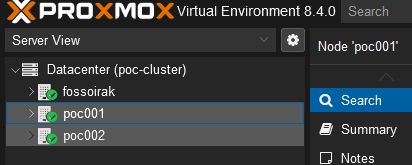
\includegraphics[width=0.85\textwidth]{../poc/cluster-info-prox.png}
%   \caption{Clusteropstelling in Proxmox VE}
%   \label{fig:cluster-proxmox}
% \end{figure}
% \subsection{Storage in Proxmox VE}
% Proxmox VE ondersteunt verschillende soorten storage. In de proof of concept is er gekozen om te werken met een CEPH storage als distributed storage. Dit is een open-source software-defined storage oplossing die kan worden gebruikt in combinatie met Proxmox VE.
% Om deze te configureren moeten er minimaal 3 schijven/partities zijn. Voor deze POC is er besloten om op elke fysieke node een fysieke schijf toe te kennen aan de CEPH storage. Dit zijn 3 willekeurige harde schijven.
% Via de GUI kan vanaf elke node worden doorgeklikt naar Ceph. Daar moet worden aangeduid welke schijf gebruikt zal worden voor de Ceph-storage. Dit kan ook via de command line.
% Nadat de schijven op elke node zijn toegevoegd, kan via het OSD-menu in de Proxmox-GUI een overzicht worden bekeken, zoals te zien is in figuur \ref{fig:osd-ceph-proxmox}.
% \begin{figure}[H]
%   \centering
%   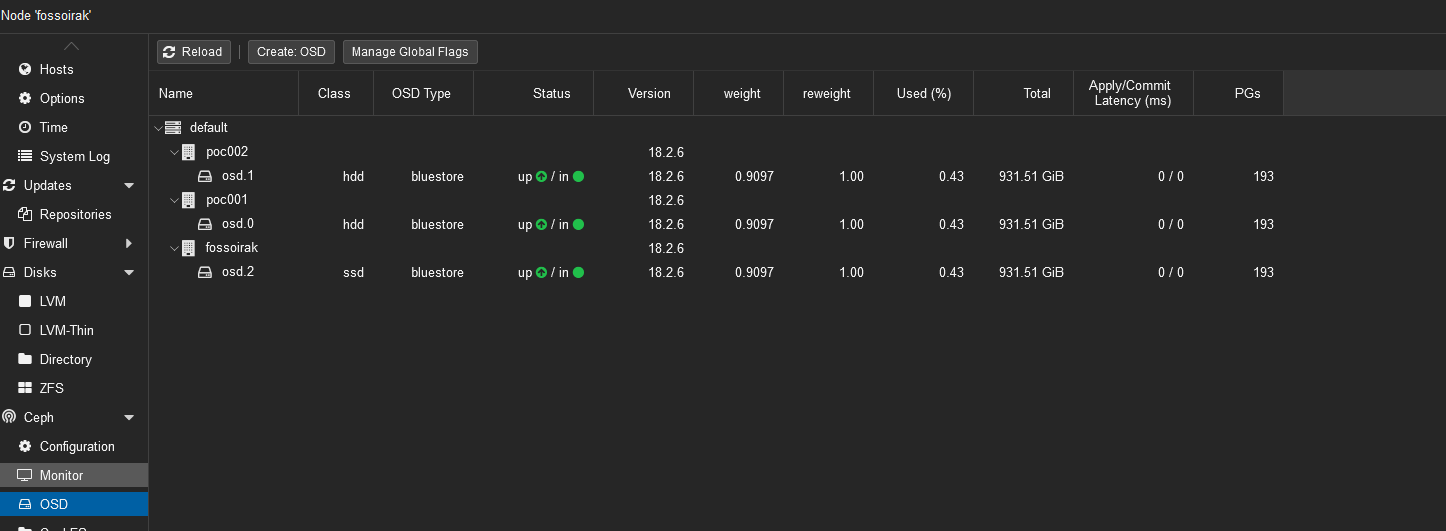
\includegraphics[width=1.2\textwidth]{../poc/ceph-osd-prox.png}
%   \caption{CEPH schijven opstelling in Proxmox VE}
%   \label{fig:osd-ceph-proxmox}
% \end{figure}

% Nu kan er een pool aangemaakt worden voor de CEPH storage. Hierin wordt het belangrijste deel van de CEPH configuratie gedaan.
% Je geeft aan hoeveel schijven er in de pool moeten zitten. Minimaal is dit hier 3 aangezien we weer met het HA systeem zitten. Om de HA regels te volgen is het ook essentieel dat er op elke fysieke node een schijf zit voor de pool.
% Bij het gebruik van Ceph in Proxmox VE moet het systeem weten hoeveel schijven minimaal beschikbaar moeten zijn om de opslagpool operationeel te houden. Voor deze POC wordt dit ingesteld op 2. Dit is ook de reden waarom er met 3 fysieke nodes is gewerkt. Bij een node failure kan de pool nog steeds gebruikt worden.
% De Crush rule in de configuratie is ook belangrijk. Dit is de manier waarop de data verdeeld wordt over de verschillende schijven. Hierin kan ook worden aangegeven dat er een replica van de data op een andere node moet worden gemaakt. Bij een node failure kan de data nog steeds worden benaderd via de andere nodes.
% De firguur \ref{fig:ceph-pool-prox} toont de huidige configuratie van de pool in Proxmox VE.
% \begin{figure}[H]
%   \centering
%   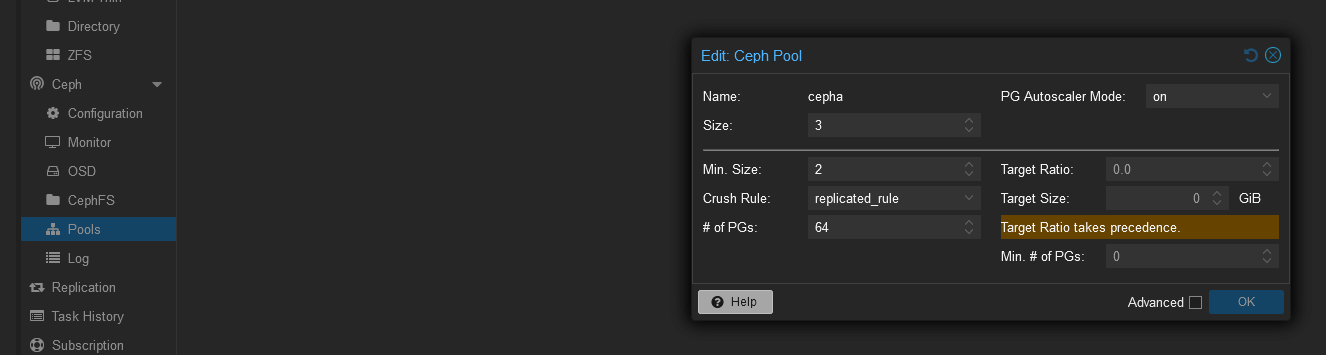
\includegraphics[width=1.1\textwidth]{../poc/ceph-pool-prox.png}
%   \caption{Pool opstelling van CEPH in Proxmox VE}
%   \label{fig:ceph-pool-prox}
% \end{figure}

% Eenmaal aangemaakt kan er een virtuele machine worden aangemakt. Deze virtuele zal Ubuntu 22.04 worden gebruikt als operating system.
% De meeste instellingen kunnen helemaal naar keuze worden ingesteld en is voor de rest buiten de scope van deze bachelorproef. De meest relevante instellingen zijn die rond de storage.
% Tijdens het configureren van de virtuele machine kan de gewenste schijf worden geselecteerd. Hierbij kan ook de eerder aangemaakte pool worden gekozen.
% Merk verder op dat er al een optie is voor SAN iSCSI met TrueNAS~\autocite{truenas} . Deze optie mag tijdelijk genegeerd worden.
% Als alles correct is verlopen, kan op alle drie de nodes naar keuze een virtuele machine worden aangemaakt, waarbij overal dezelfde optie beschikbaar is om Ceph als schijfopslag te gebruiken.
% Figuur \ref{fig:vm-storage-proxmox} toont de configuratie van de virtuele machine in Proxmox VE.
% \begin{figure}[H]
%   \centering
%   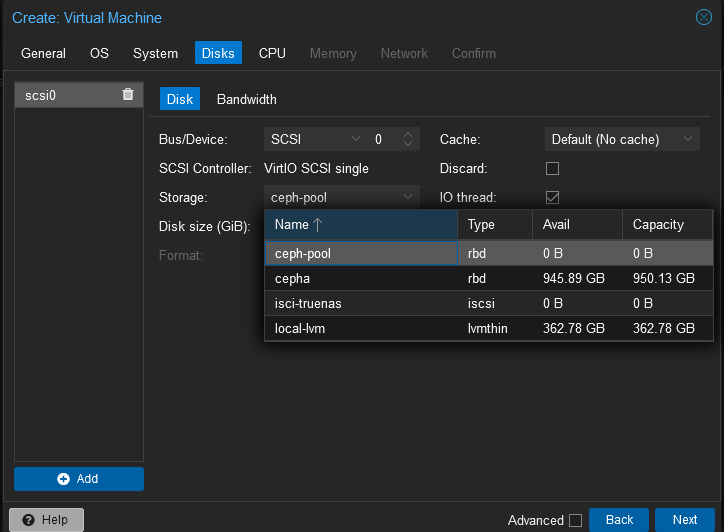
\includegraphics[width=0.85\textwidth]{../poc/vm-storage-prox.png}
%   \caption{VM configuratie met correcte disk in Proxmox VE}
%   \label{fig:vm-storage-proxmox}
% \end{figure}

% De virtuele machine is nu aangemaakt op de node fossoirak.
% Ter controle kan er in de GUI onder Datacenter bij de optie CEPH gekeken worden of alle schijven en nodes die de CEPH pool draaien healthy zijn. Zie figur \ref{fig:ceph-healthy-prox}.
% Als er geen rode kruisjes staan bij de schijven en nodes is alles perfect geconfigureerd.
% \begin{figure}[H]
%   \centering
%   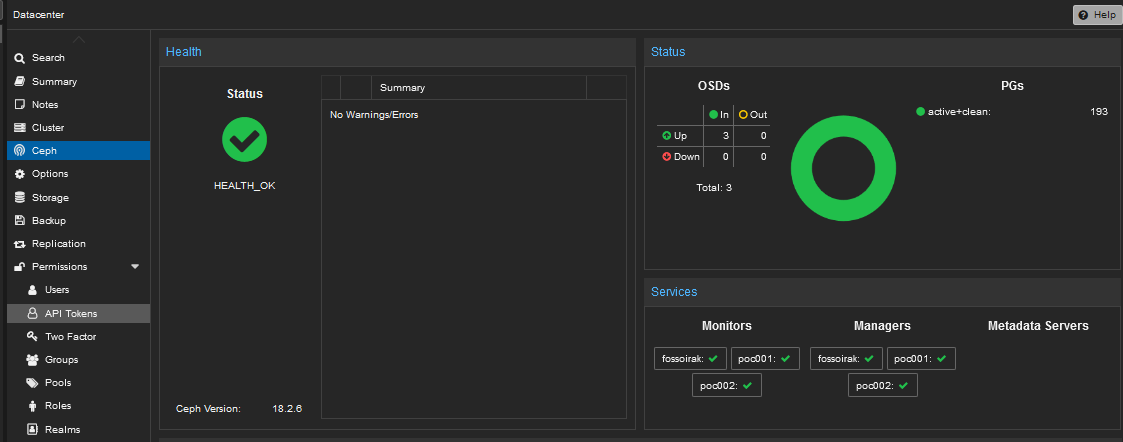
\includegraphics[width=0.85\textwidth]{../poc/ceph-healthy-prox.png}
%   \caption{de gezondheid van CEPH  in Proxmox VE}
%   \label{fig:ceph-healthy-prox}
% \end{figure}

% Hierna kan er een HA test uitgevoerd worden. Dit wordt later besproken.
% Tijdens het werken met Proxmox VE valt er op dat Proxmox VE automatisch een direct attach storage mount aanmaakt voor te gebruiken. Deze wordt gekoppeld als een directory met als naam local.
% Dit toont aan dat Proxmox VE standaard een integratie biedt met DAS. In deze situatie draait het direct op de schijf waar de Proxmox VE zelf op draait zoals te zien is in de figuur \ref{fig:das-prox}.
% \begin{figure}[H]
%   \centering
%   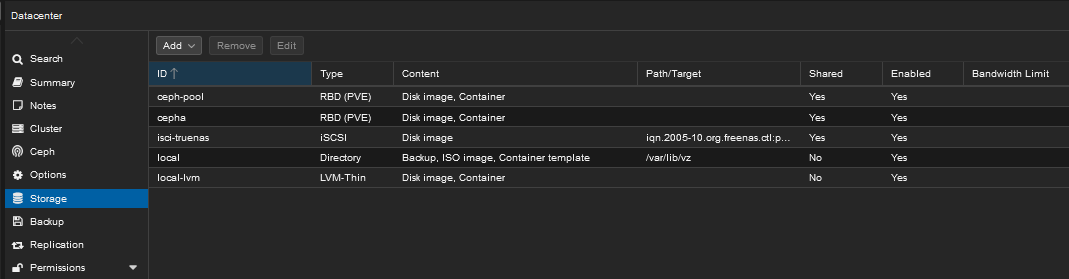
\includegraphics[width=1.1\textwidth]{../poc/das-proxmox.png}
%   \caption{direct attach storage in Proxmox VE}
%   \label{fig:das-prox}
% \end{figure}


% Nu we weten dat CEPH goed werkt moet er gekeken worden naar de SAN configuratie met ISCSI.
% Er is een bestaande TrueNAS ~\autocite{truenas} server die al draait in de omgeving. Hierop draait een block storage waar iSCI is geconfigureerd.
% Onder de tab storage bij Datacenter kan er zeer eenvoudig een iSCSI target worden aangemaakt bij Add, zie figuur \ref{fig:iscsi-SAN}.
% Via de opties in het menu moet er een correct ID als naam worden gegeven en via portal het correct IP adres van de TrueNAS service.
% Omdat er gewerkt wordt met een SAN principe staat het default bij de optie node in de configuratie op all nodes. Dit is ook de bedoeling aangezien we met een HA cluster werken.
% De configuratie van iSCI op TrueNAS is buiten de scope van deze bachelorproef.
% \begin{figure}[H]
%   \centering
%   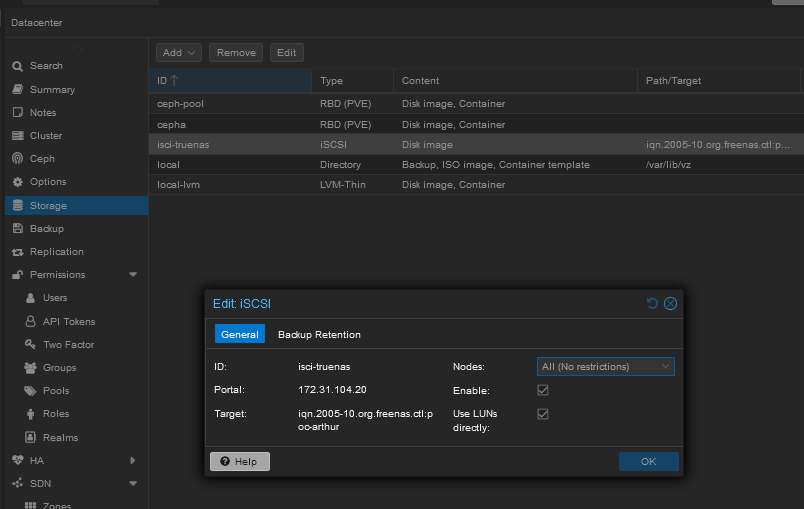
\includegraphics[width=0.85\textwidth]{../poc/iscsi-prox.png}
%   \caption{storage area network met ISCI in Proxmox VE}
%   \label{fig:iscsi-SAN}
% \end{figure}
% Nu zal er een extra  optie bijgekomen zijn in de GUI onder de tab storage bij datacenter, zie fiuur~\ref{fig:vm-lijst}  Hier in het voorbeeld wordt het al naam iSCI-TrueNAS gegeven.
% Nu maken we een 2de virtuele machine aan met dezelfde configuratie als de eerste virtuele machine maar met een andere disk. Er wordt nu gekozen voor de isci-truenas disk.
% \begin{figure}[H]
%   \centering
%   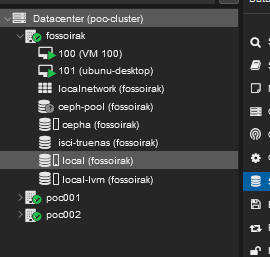
\includegraphics[width=0.85\textwidth]{../poc/vm-lijst-prox.png}
%   \caption{Lijst van de 2 virtuele machines in Proxmox VE}
%   \label{fig:vm-lijst}
% \end{figure}
% Aangezien een SAN princiepe via een vebrinding werkt op het netwerk is de storage de zwakste schakel in een high availability cluster. Deze verbinding kan verbroken worden door netwerk problemen. Hierna kan er data corruptie onstaan in het slechtste geval.

% \subsection{High Availability in Proxmox VE}

% Eenmaal de storage in orde is voor de virtuele machines kan er een HA configuratie worden aangemaakt. 
% Onder datacenter HA kan een groep worden aangemaakt. Hierin worden alle drie de fysieke nodes opgenomen die deel uitmaken van de cluster. Vervolgens wordt aan de groep een logische naam toegekend, in dit geval ha-pool zoals in figuur \ref{fig:ha-group}.
% \begin{figure}[H]
%   \centering
%   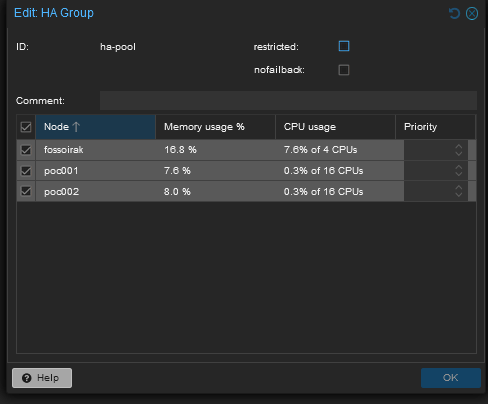
\includegraphics[width=0.85\textwidth]{../poc/ha-group.png}
%   \caption{high Availability group in Proxmox VE}
%   \label{fig:ha-group}
% \end{figure}
% Nu voegen we de 2 virtuele machines toe aan de HA groep. Dit wordt gedaan via de HA section in datancer.
% Bij Max Restart en Max Relocate wordt ingesteld hoe vaak een virtuele machine opnieuw mag worden opgestart of verplaatst naar een andere node. In dit geval moet dit groter zijn dan 0 zoals bij firguur \ref{fig:ha-vm}.
% \begin{figure}[H]
%   \centering
%   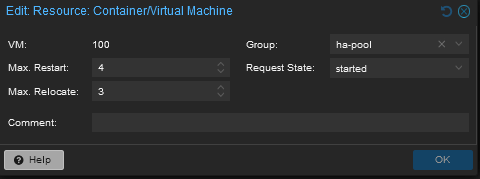
\includegraphics[width=0.85\textwidth]{../poc/vm-ha.png}
%   \caption{High Availability vm toevoegen in Proxmox VE}
%   \label{fig:ha-vm}
% \end{figure}
% Zodra beide virtuele machines aan de HA-groep zijn toegevoegd, kan de HA-configuratie worden getest.

% Om HA te testen in combinatie met beide storage systemen zal er een netwerk probleem worden gesimuleerd.
% Alle virtuele machines draaien nu op node 001
% Op de fysieke node poc001 zal de internet kabel worden uitgetrokken. Hierna kijken we hoelang het duurt vooraleer de virtuele machines opnieuw worden opgestart op een andere node, alsookop welke node specifiek.

% Figuur \ref{fig:failover-vm} kan er duidelijk gezien worden dat de virtuele machines volledig van cold mode moeten opstarten. Dit is een andere situatie dan wanneer er een migratie gedaan wordt.
% Dan wordt live de virtuele machine van de ene node naar de andere gemigreerd zonder echte downtime.
% Het systeem in Proxmox VE is nu zo ingesteld dat bij een echte failover de schade van downtime relatief beperkt blijft. Dit staat uiteraard los van data verlies die kan optreden bij een failover.
% \begin{figure}[H]
%   \centering
%   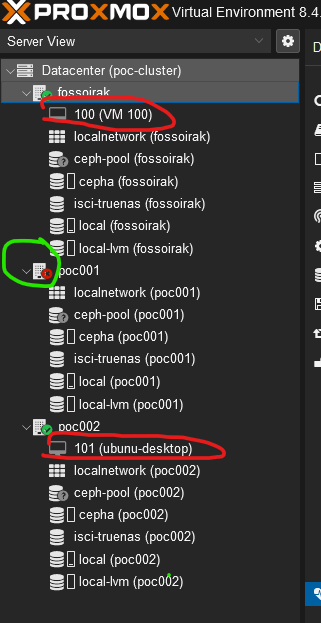
\includegraphics[width=0.85\textwidth]{../poc/failover-prox.png}
%   \caption{failover node virtuale machines herstellen in HA in Proxmox VE}
%   \label{fig:failover-vm}
% \end{figure}

% Van zodra de connectie van poc001 verboken is met de nadere nodes duurt het ongeveer 30-60 seconden vooraleer de virtuele machines opnieuw worden opgestart op een andere node. Dit is ook de tijd die nodig is om de heartbeat van de cluster te verliezen.
% Hierbij kunenn we vanuit gaan dat de default healthy check van de cluster en zijn nodes ook rond deze tijdsduur ligt. Beide virtuele machines worden opnieuw opgestart op de node foissarak en poc002. 
% Aangezien beide virtuele machines dezelfde HA group hebben, krijgen ze ook dezelfde prioriteit.

% Merk op dat zowel de virtuele machine met een SAN als de virtuele machine met een distributed storage opnieuw worden opgestart op de node foissarak. Dit toont aan dat Proxmox VE goed werkt met beide storage systemen, zeker met failover situaties.


% \subsection{Virtuele machines migraties in Proxmox VE}
% In het het werkveld komt het geregeld voor dat een node een gepland onderhoud heeft. Dit kan zijn dat er een update moet worden uitgevoerd of dat er hardware moet worden vervangen.
% Bij deze is het gewenst om te weten of er een mogelijkheid is om de virtuele machines te migreren naar een andere node zonder dat er downtime/minimale downtime is.
% Via de GUI in Proxmox VE kan een virtuele machine eenvoudig worden gemigreerd via de optie Migration rechtsboven, zodra een virtuele machine is geselecteerd, zie figuur \ref{fig:migratie-vm}.
% \begin{figure}[H]
%   \centering
%   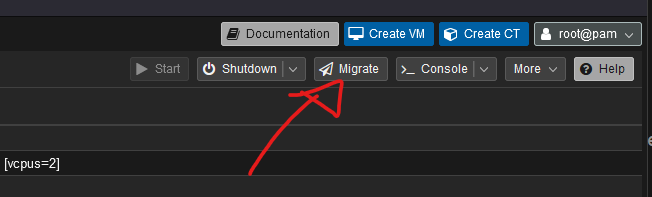
\includegraphics[width=0.85\textwidth]{../poc/vm-migratie-prox.png}
%   \caption{migratie virtuele machine in Proxmox VE}
%   \label{fig:migratie-vm}
% \end{figure}
% Tijdens het migreren van de virtuele machine blijft de console open staan van de virtuele machine. Hierbij is er een zeer korte freeze in het beeld waarna de activiteiten in de vm weer verder werken. Het totale proces voor beide virtuele machines individueel was ongeveer 30 seconden.
% Hieruit kan er bekeken worden dat de downtime bij migratie zo goed als minimaal is, wat ideaal is voor het offline brengen van een node voor bijvoorbeeld een gepland onderhoud.


% \subsection{Hot swapping fysieke disks in Proxmox VE}
% Proxmox VE biedt ook hot swapping aan van de fysieke disks. 
% Voor deze test is er een fysieke disk voor node poc002 toegevoegd, zie figuur \ref{fig:hotdisk-swap}.
% \begin{figure}[H]
%   \centering
%   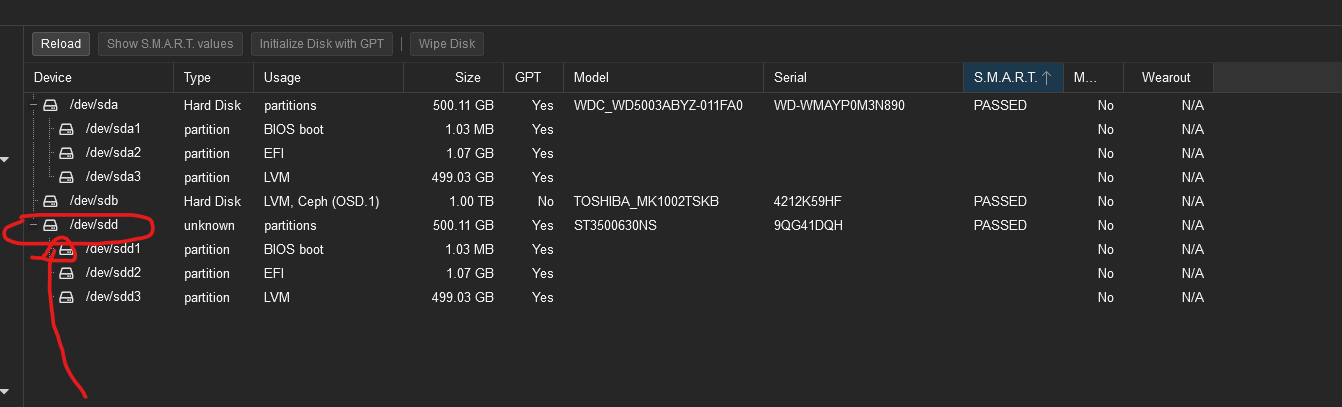
\includegraphics[width=1.2\textwidth]{../poc/hot-disk-prox.png}
%   \caption{hot disk swap in Proxmox VE}
%   \label{fig:hotdisk-swap}
% \end{figure}
% Deze noemt sdb. Eenmaal dat deze disk is toegevoegd zou de disk moeten kunnen verwijderd worden en vervangen worden door een andere zonder dat de node poc002 offline moet worden gehaald.
% Dit wordt live getest tijden het draaien. Op deze disk draait momenteel niks. Dit is belangrijk aangezien we het vervangen van een disk simuleren. De data zou normaal op voorhand moeten verwijderd zijn van de disk.

% We voegen de nieuwe disk toe in de plaats van de andere en merken direct na 15 seconden dit op, zie figuur \ref{fig:hotdiskvervangen-swap}.
% \begin{figure}[H]
%   \centering
%   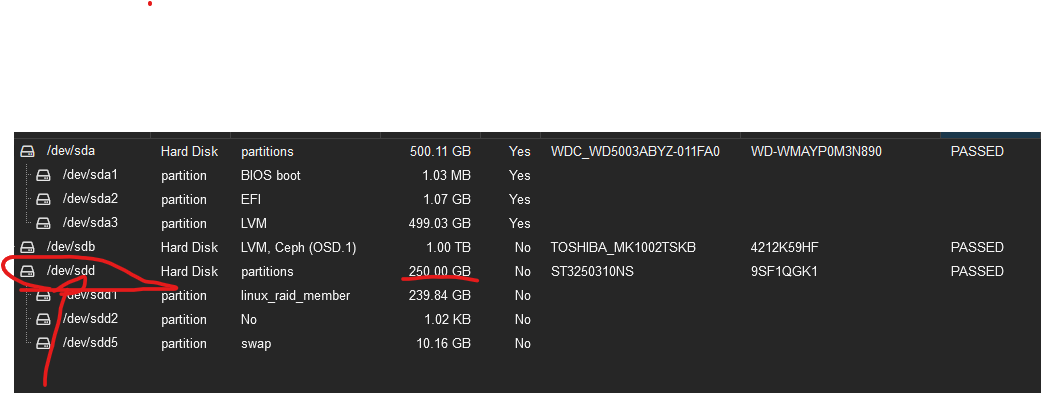
\includegraphics[width=1.2\textwidth]{../poc/hot-disktwee-prox.png}
%   \caption{hot disk swap in Proxmox VE}
%   \label{fig:hotdiskvervangen-swap}
% \end{figure}

% We zien bij figuur` \ref{fig:hotdiskvervangen-swap} dit duidelijk een andere disk is met nu een grote van 250 GB. Hiervoor was dat 500 GB.
% Voeg hier je eigen hoofdstukken toe die de ``corpus'' van je bachelorproef
% vormen. De structuur en titels hangen af van je eigen onderzoek. Je kan bv.
% elke fase in je onderzoek in een apart hoofdstuk bespreken.

%\input{...}
%\input{...}
%...

%%=============================================================================
%% Conclusie
%%=============================================================================

\chapter{Conclusie}%
\label{ch:conclusie}

% TODO: Trek een duidelijke conclusie, in de vorm van een antwoord op de
% onderzoeksvra(a)g(en). Wat was jouw bijdrage aan het onderzoeksdomein en
% hoe biedt dit meerwaarde aan het vakgebied/doelgroep? 
% Reflecteer kritisch over het resultaat. In Engelse teksten wordt deze sectie
% ``Discussion'' genoemd. Had je deze uitkomst verwacht? Zijn er zaken die nog
% niet duidelijk zijn?
% Heeft het onderzoek geleid tot nieuwe vragen die uitnodigen tot verder 
%onderzoek?

Het verwachte resultaat is een oplossing in de richting van de open-source wereld. Doordat VMware de prijzen significant verhoogt, is er een beweging ontstaan richting open-source oplossingen voor hypervisors en managementplatformen.
Hierbij ligt de focus specifiek op Proxmox VE als managementplatform met KVM als onderliggende hypervisor. Dit managementplatform is algemeen bekend en beschikt over een community met uitgebreide documentatie en support.
Het verwachte resultaat zal daarmee ook richting Proxmox VE gaan, aangezien het goedkoop in gebruik is en alvast goede ondersteuning biedt voor verschillende Linux-distributies.
De Windows-hypervisor Hyper-V biedt echter alleen ondersteuning op Windows, wat als een groot minpunt wordt beschouwd in een operationele omgeving bij Excentis.

Als dit onderzoek een objectief en goed resultaat oplevert, heeft Excentis een geschikte opvolging voor VMware, waarbij de kosten en nadelen in operationele werking zo minimaal mogelijk worden gehouden.
Hierbij wordt ook rekening gehouden met de tijd die het bedrijf kan besparen door een goede overgang naar een nieuwe managementplatformen.

%---------- Bijlagen -----------------------------------------------------------
\appendix

\chapter{proof of concept opzet}


% \section{inleiding}%
% Aan de hand van de shortlist die opgemaakt is komt er voor elke geselecteerde managementplatform een proof of concept. Hierbij wordt er gekeken hoe de nodige functionaliteiten werken en toegepast kunnen worden in het systeem.
% Belangrijk om te weten is dat de proof of concept niet de volledige functionaliteit van het managementplatform zal testen. Het doel is om een goed beeld te krijgen van de mogelijkheden en hoe deze kunnen worden toegepast binnen de infrastructuur van Excentis. 
% We verdelen alle managementplatformen in hun eigen subsecties. In deze subsecties worden dan de vooropgestelde testen op uitgevoerd.
% \section{Proxmox VE}%

% Voor deze virtual managementplatform wordt er Proxmox VE 8.4 gebruikt. Dit is de laatste versie van Proxmox VE die op dit moment beschikbaar is.
\subsection{cluster opstelling in Proxmox VE}
Voor proxmox VE is er gekozen om te werken met 3 fysieke node's. Zoals beschreven op de officiële documentatiepagina van Proxmox ondersteunt het platform high availability clustering maar moeten er minimaal 3 nodes in de cluster draaien ~\autocite{proxmoxHA}.
Hierbij spreken we over minimaal 50\% van de nodes die moeten draaien om de cluster operationeel te houden. Dit is ook de reden waarom er voor 3 nodes is gekozen.
Bij 2 nodes zou er bij een node failure geen quorum zijn en zou de cluster niet meer operationeel zijn. Dit wil zeggen dat er geen 50\% meerderheid is van de cluster die online is. Enkel bij 3 nodes kan er 1 node uitvallen en alsnog meer dan 50 procent online hebben. In zo een gavel spreken we van een quorum.
In de figuur \ref{fig:cluster-proxmox} wordt de opstelling getoond. Elke node heeft zijn unieke naam in de cluster, vaak is dat de hostname zelf.
\begin{figure}[H]
  \centering
  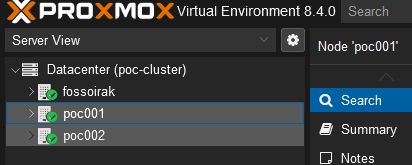
\includegraphics[width=0.85\textwidth]{../poc/cluster-info-prox.png}
  \caption{Clusteropstelling in Proxmox VE}
  \label{fig:cluster-proxmox}
\end{figure}
\subsection{Storage in Proxmox VE}
\label{sec:storage_proxmox}
Proxmox VE ondersteunt verschillende soorten storage. In de proof of concept is er gekozen om te werken met een CEPH storage als distributed storage. Dit is een open-source software-defined storage oplossing die kan worden gebruikt in combinatie met Proxmox VE.
Om deze te configureren moeten er minimaal 3 schijven/partities zijn. Voor deze POC is er besloten om op elke fysieke node een fysieke schijf toe te kennen aan de CEPH storage. Dit zijn 3 willekeurige harde schijven.
Via de GUI kan vanaf elke node worden doorgeklikt naar Ceph. Daar moet worden aangeduid welke schijf gebruikt zal worden voor de Ceph-storage. Dit kan ook via de command line.
Nadat de schijven op elke node zijn toegevoegd, kan via het OSD-menu in de Proxmox-GUI een overzicht worden bekeken, zoals te zien is in figuur \ref{fig:osd-ceph-proxmox}.
\begin{figure}[H]
  \centering
  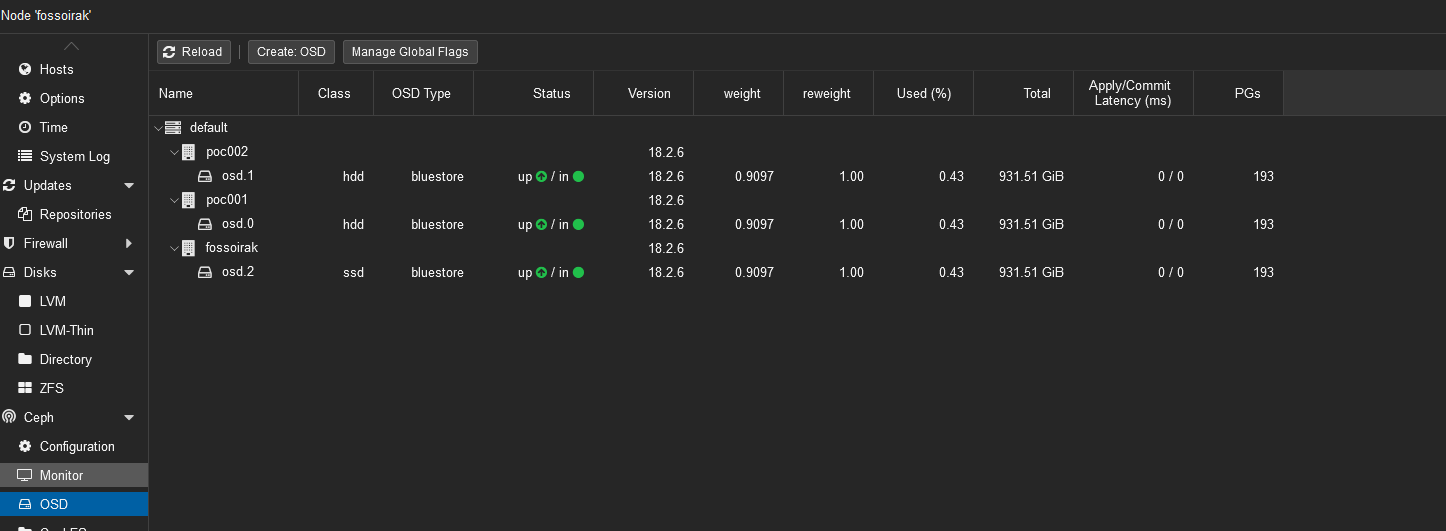
\includegraphics[width=1.2\textwidth]{../poc/ceph-osd-prox.png}
  \caption{CEPH schijven opstelling in Proxmox VE}
  \label{fig:osd-ceph-proxmox}
\end{figure}

Nu kan er een pool aangemaakt worden voor de CEPH storage. Hierin wordt het belangrijste deel van de CEPH configuratie gedaan.
Je geeft aan hoeveel schijven er in de pool moeten zitten. Minimaal is dit hier 3 aangezien we weer met het HA systeem zitten. Om de HA regels te volgen is het ook essentieel dat er op elke fysieke node een schijf zit voor de pool.
Bij het gebruik van Ceph in Proxmox VE moet het systeem weten hoeveel schijven minimaal beschikbaar moeten zijn om de opslagpool operationeel te houden. Voor deze POC wordt dit ingesteld op 2. Dit is ook de reden waarom er met 3 fysieke nodes is gewerkt. Bij een node failure kan de pool nog steeds gebruikt worden.
De Crush rule in de configuratie is ook belangrijk. Dit is de manier waarop de data verdeeld wordt over de verschillende schijven. Hierin kan ook worden aangegeven dat er een replica van de data op een andere node moet worden gemaakt. Bij een node failure kan de data nog steeds worden benaderd via de andere nodes.
De firguur \ref{fig:ceph-pool-prox} toont de huidige configuratie van de pool in Proxmox VE.
\begin{figure}[H]
  \centering
  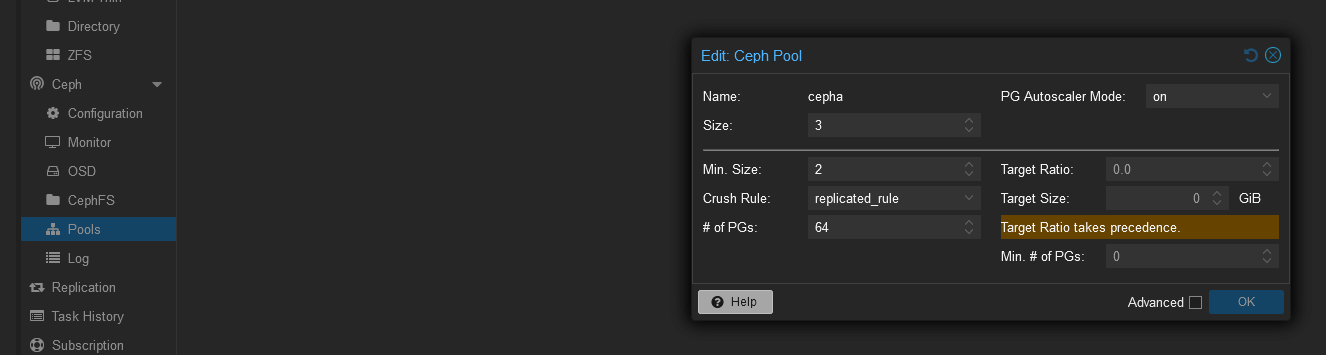
\includegraphics[width=1.1\textwidth]{../poc/ceph-pool-prox.png}
  \caption{Pool opstelling van CEPH in Proxmox VE}
  \label{fig:ceph-pool-prox}
\end{figure}

Eenmaal aangemaakt kan er een virtuele machine worden aangemakt. Deze virtuele zal Ubuntu 22.04 worden gebruikt als operating system.
De meeste instellingen kunnen helemaal naar keuze worden ingesteld en is voor de rest buiten de scope van deze bachelorproef. De meest relevante instellingen zijn die rond de storage.
Tijdens het configureren van de virtuele machine kan de gewenste schijf worden geselecteerd. Hierbij kan ook de eerder aangemaakte pool worden gekozen.
Merk verder op dat er al een optie is voor SAN iSCSI met TrueNAS~\autocite{truenas} . Deze optie mag tijdelijk genegeerd worden.
Als alles correct is verlopen, kan op alle drie de nodes naar keuze een virtuele machine worden aangemaakt, waarbij overal dezelfde optie beschikbaar is om Ceph als schijfopslag te gebruiken.
Figuur \ref{fig:vm-storage-proxmox} toont de configuratie van de virtuele machine in Proxmox VE.
\begin{figure}[H]
  \centering
  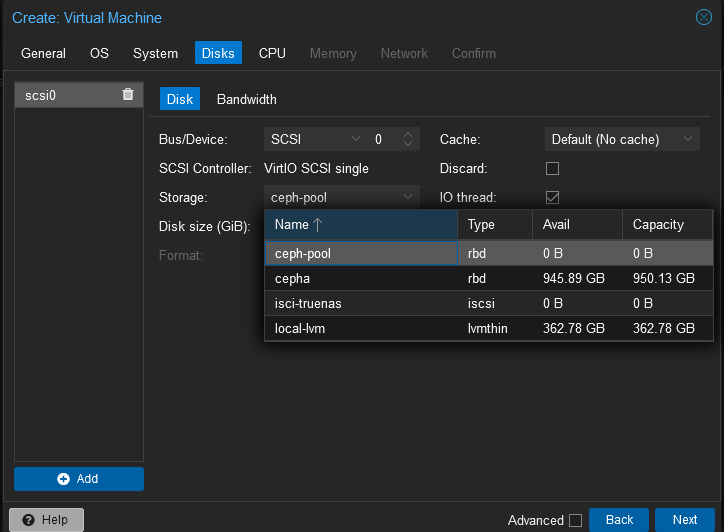
\includegraphics[width=0.85\textwidth]{../poc/vm-storage-prox.png}
  \caption{VM configuratie met correcte disk in Proxmox VE}
  \label{fig:vm-storage-proxmox}
\end{figure}

De virtuele machine is nu aangemaakt op de node fossoirak.
Ter controle kan er in de GUI onder Datacenter bij de optie CEPH gekeken worden of alle schijven en nodes die de CEPH pool draaien healthy zijn. Zie figur \ref{fig:ceph-healthy-prox}.
Als er geen rode kruisjes staan bij de schijven en nodes is alles perfect geconfigureerd.
\begin{figure}[H]
  \centering
  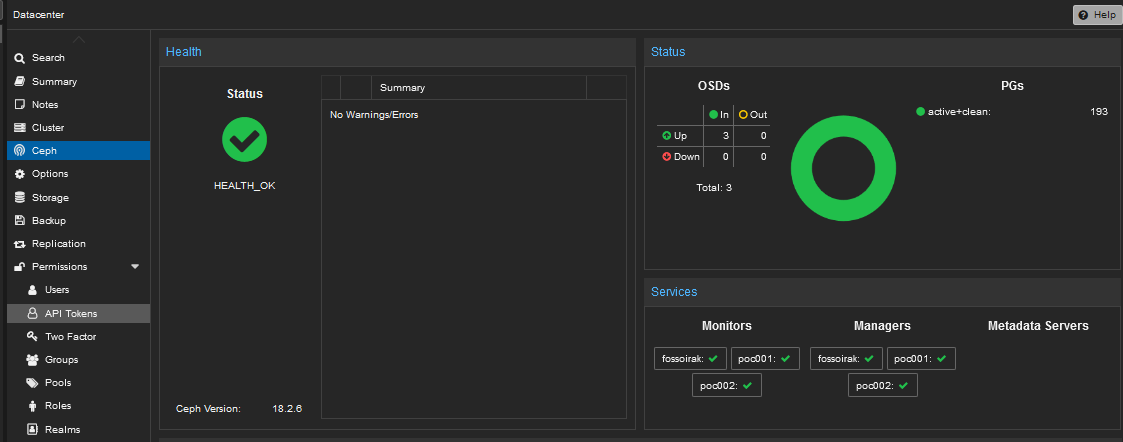
\includegraphics[width=1.1\textwidth]{../poc/ceph-healthy-prox.png}
  \caption{de gezondheid van CEPH  in Proxmox VE}
  \label{fig:ceph-healthy-prox}
\end{figure}

Hierna kan er een HA test uitgevoerd worden. Dit wordt later besproken.
Tijdens het werken met Proxmox VE valt er op dat Proxmox VE automatisch een direct attach storage mount aanmaakt voor te gebruiken. Deze wordt gekoppeld als een directory met als naam local.
Dit toont aan dat Proxmox VE standaard een integratie biedt met DAS. In deze situatie draait het direct op de schijf waar de Proxmox VE zelf op draait zoals te zien is in de figuur \ref{fig:das-prox}.
\begin{figure}[H]
  \centering
  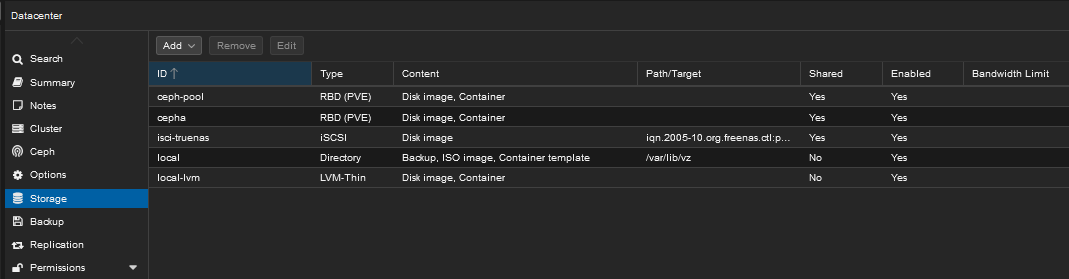
\includegraphics[width=1.2\textwidth]{../poc/das-proxmox.png}
  \caption{direct attach storage in Proxmox VE}
  \label{fig:das-prox}
\end{figure}


Nu we weten dat CEPH goed werkt moet er gekeken worden naar de SAN configuratie met ISCSI.
Er is een bestaande TrueNAS ~\autocite{truenas} server die al draait in de omgeving. Hierop draait een block storage waar iSCI is geconfigureerd.
Onder de tab storage bij Datacenter kan er zeer eenvoudig een iSCSI target worden aangemaakt bij Add, zie figuur \ref{fig:iscsi-SAN}.
Via de opties in het menu moet er een correct ID als naam worden gegeven en via portal het correct IP adres van de TrueNAS service.
Omdat er gewerkt wordt met een SAN principe staat het default bij de optie node in de configuratie op all nodes. Dit is ook de bedoeling aangezien we met een HA cluster werken.
De configuratie van iSCI op TrueNAS is buiten de scope van deze bachelorproef.
\begin{figure}[H]
  \centering
  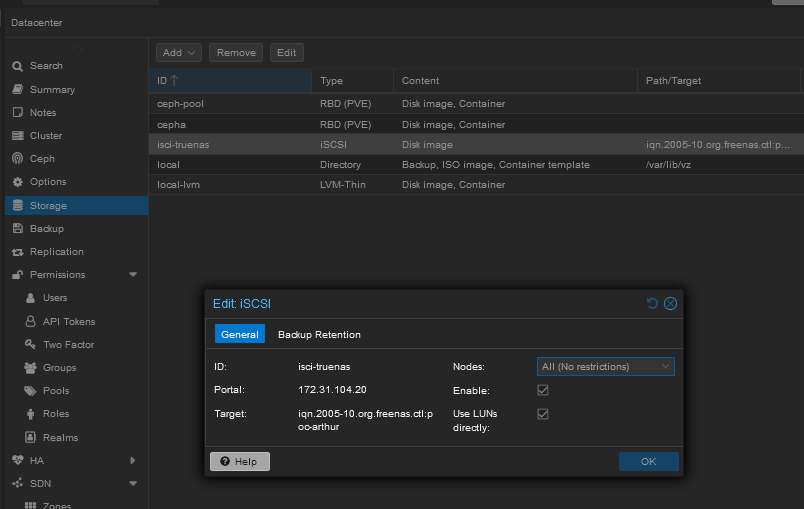
\includegraphics[width=1.1\textwidth]{../poc/iscsi-prox.png}
  \caption{storage area network met ISCI in Proxmox VE}
  \label{fig:iscsi-SAN}
\end{figure}
Nu zal er een extra  optie bijgekomen zijn in de GUI onder de tab storage bij datacenter, zie fiuur~\ref{fig:vm-lijst}  Hier in het voorbeeld wordt het al naam iSCI-TrueNAS gegeven.
Nu maken we een 2de virtuele machine aan met dezelfde configuratie als de eerste virtuele machine maar met een andere disk. Er wordt nu gekozen voor de isci-truenas disk.
\begin{figure}[H]
  \centering
  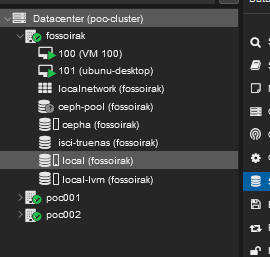
\includegraphics[width=0.85\textwidth]{../poc/vm-lijst-prox.png}
  \caption{Lijst van de 2 virtuele machines in Proxmox VE}
  \label{fig:vm-lijst}
\end{figure}
Aangezien een SAN princiepe via een vebrinding werkt op het netwerk is de storage de zwakste schakel in een high availability cluster. Deze verbinding kan verbroken worden door netwerk problemen. Hierna kan er data corruptie onstaan in het slechtste geval.

\subsection{High Availability in Proxmox VE}
\label{sec:ha-proxmox}
Eenmaal de storage in orde is voor de virtuele machines kan er een HA configuratie worden aangemaakt. 
Onder datacenter HA kan een groep worden aangemaakt. Hierin worden alle drie de fysieke nodes opgenomen die deel uitmaken van de cluster. Vervolgens wordt aan de groep een logische naam toegekend, in dit geval ha-pool zoals in figuur \ref{fig:ha-group}.
\begin{figure}[H]
  \centering
  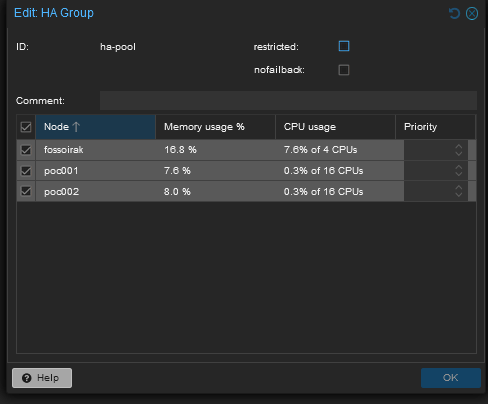
\includegraphics[width=0.85\textwidth]{../poc/ha-group.png}
  \caption{high Availability group in Proxmox VE}
  \label{fig:ha-group}
\end{figure}
Nu voegen we de 2 virtuele machines toe aan de HA groep. Dit wordt gedaan via de HA section in datancer.
Bij Max Restart en Max Relocate wordt ingesteld hoe vaak een virtuele machine opnieuw mag worden opgestart of verplaatst naar een andere node. In dit geval moet dit groter zijn dan 0 zoals bij firguur \ref{fig:ha-vm}.
\begin{figure}[H]
  \centering
  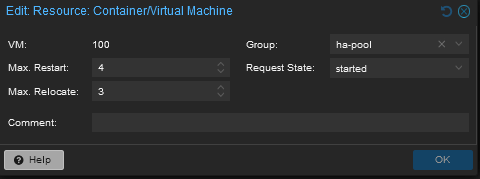
\includegraphics[width=0.85\textwidth]{../poc/vm-ha.png}
  \caption{High Availability vm toevoegen in Proxmox VE}
  \label{fig:ha-vm}
\end{figure}
% Ik heb dit verplaatst naar poc




\begin{figure}[H]
  \centering
  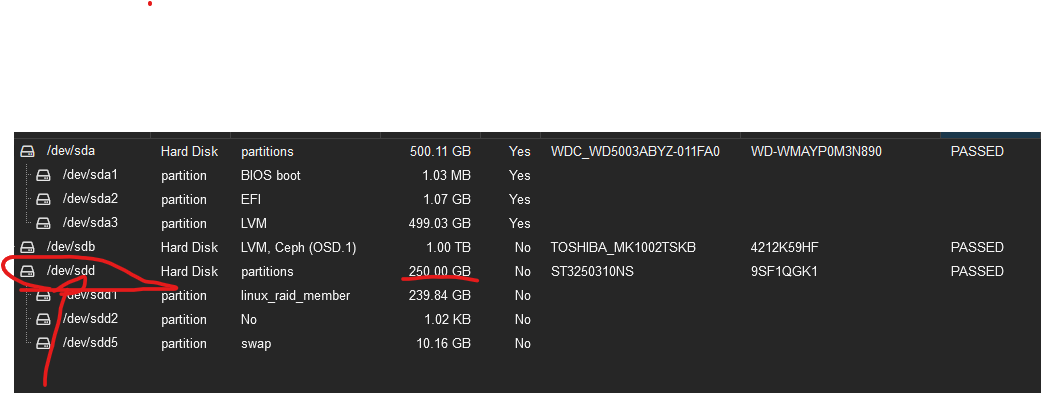
\includegraphics[width=1.2\textwidth]{../poc/hot-disktwee-prox.png}
  \caption{hot disk swap in Proxmox VE}
  \label{fig:hotdiskvervangen-swap}
\end{figure}

We zien bij figuur` \ref{fig:hotdiskvervangen-swap} dit duidelijk een andere disk is met nu een grote van 250 GB. Hiervoor was dat 500 GB.

\appendix

\chapter{Onderzoeksvoorstel}

Het onderwerp van deze bachelorproef is gebaseerd op een onderzoeksvoorstel dat vooraf werd beoordeeld door de promotor. Dat voorstel is opgenomen in deze bijlage.

%% TODO: 
%\section*{Samenvatting}

% Kopieer en plak hier de samenvatting (abstract) van je onderzoeksvoorstel.

% Verwijzing naar het bestand met de inhoud van het onderzoeksvoorstel
%---------- Inleiding ---------------------------------------------------------

% TODO: Is dit voorstel gebaseerd op een paper van Research Methods die je
% vorig jaar hebt ingediend? Heb je daarbij eventueel samengewerkt met een
% andere student?
% Zo ja, haal dan de tekst hieronder uit commentaar en pas aan.

%\paragraph{Opmerking}

% Dit voorstel is gebaseerd op het onderzoeksvoorstel dat werd geschreven in het
% kader van het vak Research Methods dat ik (vorig/dit) academiejaar heb
% uitgewerkt (met medesturent VOORNAAM NAAM als mede-auteur).
% 

\section{Inleiding}%
\label{sec:inleiding}

Door de aankondiging van VMware om de licentiekosten te verhogen~\autocite{device42_2024}, zijn er bedrijven die beginnen te denken aan een eventueel alternatief voor VMware ESXi/VMWare vCenter.
De prijzen voor deze software zijn zo hoog~\autocite{Hale2024} dat bedrijven zoeken naar alternatieven.
Vaak gaat het om bedrijven die virtualisatie hebben als een service, waarbij dit niet de allerbelangrijkste zorg is binnen het bedrijf.
VMware-producten zit hard vastgeworteld in bedrijven doordat ze werken met verschillende automatisatietools en scripts. Zo'n overgang naar een nieuwe managementplatform zal een impact hebben op elke IT-infrastructuur.
Om deze overgang ook vloeiend te kunnen laten lopen, moet er in de managementplatform ook ondersteuning zijn voor deze verschillende tools.
De mensen binnen IT moeten hierbij ook een omscholing krijgen of zich gaan verdiepen in de managementplatformen  voor virtualisatie. De documentatie en support/community achter de managementplatformen is zeker een aspect dat in rekening moet worden genomen.
Deze bachelorproef richt zich op het bedrijf Excentis: Welke alternatieven zijn er om het huidige VMware vCenter te vervangen en hoe kan die passen binnen de noden van omgeving van Excentis?
De volgende vragen moeten wij ons stellen bij het zoeken naar alternatieven op de markt.
\begin{enumerate}
\item Welke functionele en prestatieverschillen zijn er tussen open-source en closed-source managementplatformen, en welke voor- en nadelen hebben deze verschillen voor het bedrijf Excentis?
\item In welke mate integreren managementplatformen met tools zoals Nakivo, Ansible en Foreman, en hoe kunnen deze toegepast worden binnen Excentis?
\item Hoe presteren managementplatformen op het gebied van High Availability(failover,\newline schaalbaarheid,backups,...)?
\item Hoe kan de bestaande ondersteuning van Direct Attached Storage en Serial Attached SCSI in VMWare vCenter worden overgezet naar een alternatief managementplatformen binnen de infrastructuur van Excentis?
\item Op welke manier is er een mogelijkheid om de bestaande managementplatformen omgeving van Excentis over te zetten naar het nieuwe alternatief?
\end{enumerate}



% Waarover zal je bachelorproef gaan? Introduceer het thema en zorg dat volgende zaken zeker duidelijk aanwezig zijn:

% \begin{itemize}
%   \item kaderen thema
%   \item de doelgroep
%   \item de probleemstelling en (centrale) onderzoeksvraag
%   \item de onderzoeksdoelstelling
% \end{itemize}

% Denk er aan: een typische bachelorproef is \textit{toegepast onderzoek}, wat betekent dat je start vanuit een concrete probleemsituatie in bedrijfscontext, een \textbf{casus}. Het is belangrijk om je onderwerp goed af te bakenen: je gaat voor die \textit{ene specifieke probleemsituatie} op zoek naar een goede oplossing, op basis van de huidige kennis in het vakgebied.

% De doelgroep moet ook concreet en duidelijk zijn, dus geen algemene of vaag gedefinieerde groepen zoals \emph{bedrijven}, \emph{developers}, \emph{Vlamingen}, enz. Je richt je in elk geval op it-professionals, een bachelorproef is geen populariserende tekst. Eén specifiek bedrijf (die te maken hebben met een concrete probleemsituatie) is dus beter dan \emph{bedrijven} in het algemeen.

% Formuleer duidelijk de onderzoeksvraag! De begeleiders lezen nog steeds te veel voorstellen waarin we geen onderzoeksvraag terugvinden.

% Schrijf ook iets over de doelstelling. Wat zie je als het concrete eindresultaat van je onderzoek, naast de uitgeschreven scriptie? Is het een proof-of-concept, een rapport met aanbevelingen, \ldots Met welk eindresultaat kan je je bachelorproef als een succes beschouwen?

%---------- Stand van zaken ---------------------------------------------------

\section{Literatuurstudie}
\label{sec:literatuurstudie}
VMware~\autocite{vmware} is een bedrijf die zich bezighoud met alles rond virtualisatie. De sterke prijsstijgingen van VMware zorgen ervoor dat veel bedrijven afhaken en op zoek gaan naar alternatieven~\autocite{Hale2024}. Er zijn verschillende alternatieve managementplatformen met bijhorende hypervisors.

\subsection{Hypervisors}
In het huidige systeem dat Excentis gebruikt als onderliggen hypervisor is VMWARE ESXI~\autocite{vmware}. Deze is closed source en werkt binnen het VMware systeem.
Een voorbeeld hiervan is 'KVM' (Kernel-based Virtual Machine)\autocite{KVM}. KVM is open source en vrij te gebruiken voor iedereen\autocite{KVM}. Microsoft Hyper-V ~\autocite{Eaton2019} wordt ook genoemd als mogelijke vergelijking met VMware ESXI~\autocite{fayyad2013benchmarking}. Hierin wordt een vergelijking gemaakt tussen verschillende hypervisors die geselecteerd zijn.
Verder in de virtualisatie wereld hebben wij ook nog het Xen Project~\autocite{xenproject}. Dit is een open-source hypervisor die zich vooral richt op cloud computing en server virtualisatie ~\autocite{binu2011virtualization}.
XenServer~\autocite{xenserver} is ook een alternatieve software keuze voor VMware ESXI. XenServer is een commerciële hypervisor die zich richt op bedrijven en enterprise-ondersteuning biedt.

\subsection{managementplatformen}
Excentis gebruikt bovenliggend als managementplatformen VMWare vCenter~\autocite{vmware}. Deze zou dus moeten vervangen worden.
Proxmox VE~\autocite{Proxmox} is een open-source managementplatform dat werkt met KVM en enterprise-ondersteuning aanbiedt voor bedrijven. Uit dit onderzoek~\autocite{ally2018comparative} blijkt dat Proxmox, dat gebruik maakt van KVM zeker niet onderdoet tegenover andere closed source systemen.
OpenStack is een open-source cloud computing platform~\autocite{openstack2024}. Deze bied niet alleen ondersteuning voor KVM maar ook voor Xen~\autocite{oleksiuk2023comparative}.
Microsoft System Center Virtual Machine Manager (SCVMM)~\autocite{microsoftvmm2025} is van microsoft en bied een managementplatform systeem aan voor Hyper-V.
XenCenter~\autocite{xencenter2024} bied een managementplatform aan voor XenServer~\autocite{xenserver}.

\subsection{Open source systemen}
Er zijn vele soorten softwarepakketten op de markt die hypervisors en managementplatformen aanbieden. Hieruit kunnen wij ze onderverdelen in twee groepen: de closed-source en open-source hypervisors. Elke groep heeft zijn voor- en nadelen. Alles hangt steeds af van de noden en vereisten van het bedrijf of instelling.
Proxmox VE is open source~\autocite{Proxmox}. Dit wil zeggen dat de systemen kosteloos gebruikt kunnen worden. Support bij problemen valt hierbij wel af. Er is wel een mogelijkheid om bij hen een enterprise support services subscription te nemen. Hierbij kan er alsnog beroep worden gedaan bij eventuele problemen.
Open source software is een evidentie maar zorgt voor meer zelfstandig werk bij installatie en rust meer op de community achter de software.

\subsection{closed source systemen}
Andere alternatieven systemen zijn closed-source. Hierbij hebben we het onder andere over VMware ESXi/VMware vCenter~\autocite{vmware} en Microsoft Hyper-V~\autocite{Eaton2019}. Deze software systemen zijn niet gratis en vragen een licentie om te mogen gebruiken. Dit is een nadeel ten opzichte van open-source systemen.
Bij bedrijven waar stabiliteit en betrouwbaarheid hoog in het vaandel staan, zoals in een wetenschappelijke omgeving, kan het een goede keuze zijn om te kiezen voor closed-source hypervisors~\autocite{voras2012early}. Dit wil niet zeggen dat andere systemen uitgesloten zijn.
\subsection{Soorten storage systemen}
Wanneer we praten over storage in de virtualisatiewereld, dan hebben we het ook over 'Serial-Attached SCSI' (SAS) en 'Direct-Attached Storage' (DAS). Deze technologieën zorgen ervoor dat er een hoge beschikbaarheid is van de data en dat deze snel kan worden opgevraagd~\autocite{griswold2002storage}. Dit is een belangrijk aspect in de virtualisatiewereld en is een belangrijke eis voor Excentis.
SAS is een snelle, betrouwbare opslaginterface die servers en high-performance opslagapparaten verbindt~\autocite{aravindan2014performance}. Dit is een belangrijk om een consistente oplsag te garanderen. DAS is een opslagarchitectuur waarbij opslag direct fysiek is verbonden aan een enkele server, zonder tussenkomst van een netwerk. Deze technologie is goedkoper en eenvoudiger, maar garandeert niet alle voordelen die SAS wel kan garanderen~\autocite{griswold2002storage}.
DAS wordt vaak gebruikt in kleinere bedrijven waar de data niet zo belangrijk is en waar de data niet zo vaak wordt opgevraagd. SAS wordt vaak gebruikt in grotere bedrijven waar de data zeer belangrijk is en waar de data vaak wordt opgevraagd~\autocite{griswold2002storage}.
Zo goed als alle managementplatformen ondersteunen DAS en SAS in ons onderzoek. Excentis wilt weten hoe deze ondersteuning kan worden overgezet naar een nieuw managementplatform.

\subsection{High Availability-ondersteuning}
In dit onderzoek~\autocite{dudnik2017creating} wordt een grote vergelijking gedaan tussen hypervisors en hun managementplatformen. Hierin spit men toe op bepaalde aspecten binnen de term High Availability.
Er zijn verschillende aspecten die moeten worden bekeken en waaraan voldaan moet worden om aan een goede High Availability te voldoen. Een failover-systeem dat het ene systeem het andere systeem over laat nemen bij een bepaalde fout, is een van die aspecten in het onderzoek van~\autocite{dudnik2017creating}.
Op netwerkniveau moet er ook nagedacht worden over zowel schaalbaarheid bij piekmomenten als bij problemen die zich voordoen in het netwerk. Migratie tussen verschillende fysieke servers moet ook mogelijk zijn om een goede High Availability te garanderen~\autocite{dudnik2017creating}.
Workloadmanagers kunnen een goede oplossing zijn om overbelasting tegen te gaan op drukke piekmomenten. Back-ups van de data worden ook gezien als een belangrijk aspect voor High Availability.
% \subsection{KVM}
% \subsection{Microsoft Hyper-V}
% \subsection{Kernel-based Virtual Machine}
% \subsection{ProxMox VE}
% \subsection{xenproject}
% \subsection{High Availability-ondersteuning}
% \subsection{Direct Attached Storage en Serial Attached SCSI}

% Voor literatuurverwijzingen zijn er twee belangrijke commando's:
% \autocite{KEY} => (Auteur, jaartal) Gebruik dit als de naam van de auteur
%   geen onderdeel is van de zin.
% \textcite{KEY} => Auteur (jaartal)  Gebruik dit als de auteursnaam wel een
%   functie heeft in de zin (bv. ``Uit onderzoek door Doll & Hill (1954) bleek
%   ...'')


%---------- Methodologie ------------------------------------------------------
\section{Methodologie}%
\label{sec:methodologie}
Een objectief resultaat van alle managementplatformen is gewenst om deze vervolgens naast elkaar te kunnen vergelijken. Om dit te bereiken, wordt een vergelijkende studie uitgevoerd. De verschillende managementplatformen worden met elkaar vergeleken om te bepalen welke het beste aansluit bij de noden van Excentis.
Aan de hand van literatuurstudie en onderzoeken worden de managementplatformen geselecteerd die met elkaar worden vergeleken.
Er zal samen met Excentis worden overlopen welke eisen zeker voldaan moeten worden en wat het bedrijf echt nodig heeft in hun managementplatform, gecombineerd met hun bestaande infrastructuur. Er zal ook gekeken worden naar wat er momenteel allemaal wordt gebruikt binnen hun omgeving. Deze zullen dan worden meegenomen als basisvereisten voor de alternatieve managementplatformen.
De hardware en omgeving waarin alles wordt getest en opgebouwd, worden opgesteld in een testomgeving bij Excentis. Dit maakt het mogelijk om de managementplatformen te testen in een realistische omgeving, wat essentieel is om een objectief resultaat te bekomen.
Deze omgeving zal bestaan uit 2 verouderde DELL servers die in de serverruimte van Excentis staan. Hierbij zal alles op kleine schaal kunnen worden uitgevoerd.
Op deze servers worden de geselecteerde managementplatformen geïnstalleerd.
Voor de vergelijking van de managementplatformen worden de volgende acties uitgevoerd op de testomgeving van Excentis:
\begin{itemize}
\item werking met de bestaande hardware van Excentis, vergeleken op prestatie en stabiliteit. (Hoe snel start een nieuwe virtuele machine op, wat zijn de minimum eisen voor de hardware, ...).
\item Testen en meten van de performance en stabiliteit van de bestaande Direct Attached Storage en Serial Attached SCSI-systemen die Excentis gebruikt aan de hand van testdata op de nieuwe managementplatformen.
\item De integratie van bepalende systemen binnen Excentis testen, zoals CI/CD-tools, op de nieuwe managementplatformen.
\item Prestatie en stabiliteit van de managementplatformen bij piekmomenten en failovers.
\end{itemize}
Deze acties worden stap voor stap gedaan bij elke managementplatform. Deze worden gedaan om zo een zo objectief mogelijk resultaat te krijgen per managementplatform.
Als alle acties zijn uitgevoerd, worden de resultaten met elkaar vergeleken en wordt er een conclusie getrokken over welk managementplatform het beste aansluit bij de noden van Excentis.
% Hier beschrijf je hoe je van plan bent het onderzoek te voeren. Welke onderzoekstechniek ga je toepassen om elk van je onderzoeksvragen te beantwoorden? Gebruik je hiervoor literatuurstudie, interviews met belanghebbenden (bv.~voor requirements-analyse), experimenten, simulaties, vergelijkende studie, risico-analyse, PoC, \ldots?

% Valt je onderwerp onder één van de typische soorten bachelorproeven die besproken zijn in de lessen Research Methods (bv.\ vergelijkende studie of risico-analyse)? Zorg er dan ook voor dat we duidelijk de verschillende stappen terug vinden die we verwachten in dit soort onderzoek!

% Vermijd onderzoekstechnieken die geen objectieve, meetbare resultaten kunnen opleveren. Enquêtes, bijvoorbeeld, zijn voor een bachelorproef informatica meestal \textbf{niet geschikt}. De antwoorden zijn eerder meningen dan feiten en in de praktijk blijkt het ook bijzonder moeilijk om voldoende respondenten te vinden. Studenten die een enquête willen voeren, hebben meestal ook geen goede definitie van de populatie, waardoor ook niet kan aangetoond worden dat eventuele resultaten representatief zijn.

% Uit dit onderdeel moet duidelijk naar voor komen dat je bachelorproef ook technisch voldoen\-de diepgang zal bevatten. Het zou niet kloppen als een bachelorproef informatica ook door bv.\ een student marketing zou kunnen uitgevoerd worden.

% Je beschrijft ook al welke tools (hardware, software, diensten, \ldots) je denkt hiervoor te gebruiken of te ontwikkelen.

% Probeer ook een tijdschatting te maken. Hoe lang zal je met elke fase van je onderzoek bezig zijn en wat zijn de concrete \emph{deliverables} in elke fase?

%---------- Verwachte resultaten ----------------------------------------------
\section{Verwacht resultaat, conclusie}%
\label{sec:verwachte_resultaten}

Het verwachte resultaat is een oplossing in de richting van de open-source wereld. Doordat VMware de prijzen significant verhoogt, is er een beweging ontstaan richting open-source oplossingen voor hypervisors en managementplatformen.
Hierbij ligt de focus specifiek op Proxmox VE als managementplatform met KVM als onderliggende hypervisor. Deze managementplatform is algemeen bekend en beschikt over een community met uitgebreide documentatie en support.
Het verwachte resultaat zal daarmee ook richting Proxmox VE gaan, aangezien het goedkoop in gebruik is en alvast goede ondersteuning biedt voor verschillende Linux-distributies.
De Windows-hypervisor Hyper-V biedt echter alleen ondersteuning op Windows, wat als een groot minpunt wordt beschouwd in een operationele omgeving bij Excentis.

Als dit onderzoek een objectief en goed resultaat oplevert, heeft Excentis een geschikte opvolging voor VMware, waarbij de kosten en nadelen in operationele werking zo minimaal mogelijk worden gehouden.
Hierbij wordt ook rekening gehouden met de tijd die het bedrijf kan besparen door een goede overgang naar een nieuwe managementplatformen.
% Hier beschrijf je welke resultaten je verwacht. Als je metingen en simulaties uitvoert, kan je hier al mock-ups maken van de grafieken samen met de verwachte conclusies. Benoem zeker al je assen en de onderdelen van de grafiek die je gaat gebruiken. Dit zorgt ervoor dat je concreet weet welk soort data je moet verzamelen en hoe je die moet meten.

% Wat heeft de doelgroep van je onderzoek aan het resultaat? Op welke manier zorgt jouw bachelorproef voor een meerwaarde?

% Hier beschrijf je wat je verwacht uit je onderzoek, met de motivatie waarom. Het is \textbf{niet} erg indien uit je onderzoek andere resultaten en conclusies vloeien dan dat je hier beschrijft: het is dan juist interessant om te onderzoeken waarom jouw hypothesen niet overeenkomen met de resultaten.




%%---------- Andere bijlagen --------------------------------------------------
% TODO: Voeg hier eventuele andere bijlagen toe. Bv. als je deze BP voor de
% tweede keer indient, een overzicht van de verbeteringen t.o.v. het origineel.
%\input{...}

%%---------- Backmatter, referentielijst ---------------------------------------

\backmatter{}

\setlength\bibitemsep{2pt} %% Add Some space between the bibliograpy entries
\printbibliography[heading=bibintoc]

\end{document}
